
\section{Results and Discussion}\label{sec:Results}

\subsection{Phase Verification and Feasibility Outcomes}

The 16 candidate alloys selected for iteration BBA were chosen by diversity-aware k-medoids sampling across the 37 chemical subsystems (Section~2.1.3). \autoref{fig:alloy_affine_projection} shows the target chemistries of all 48 alloys synthesized in this work, projected from the 8-element composition simplex onto a regular octagon by affine coordinates and colored by iteration. This view emphasizes how the campaign progressively populated distinct regions of the accessible composition space across BBA, BBB, and BBC. A more detailed visualization of the iteration-0 batch selection is provided in the \textbf{SI}. All candidates across the three iterations were synthesized via vacuum arc melting, cold rolled, and recrystallized as described in Section~2.2. Phase purity was assessed by XRD for every alloy prior to mechanical testing.

\begin{figure}[htbp]
    \centering
    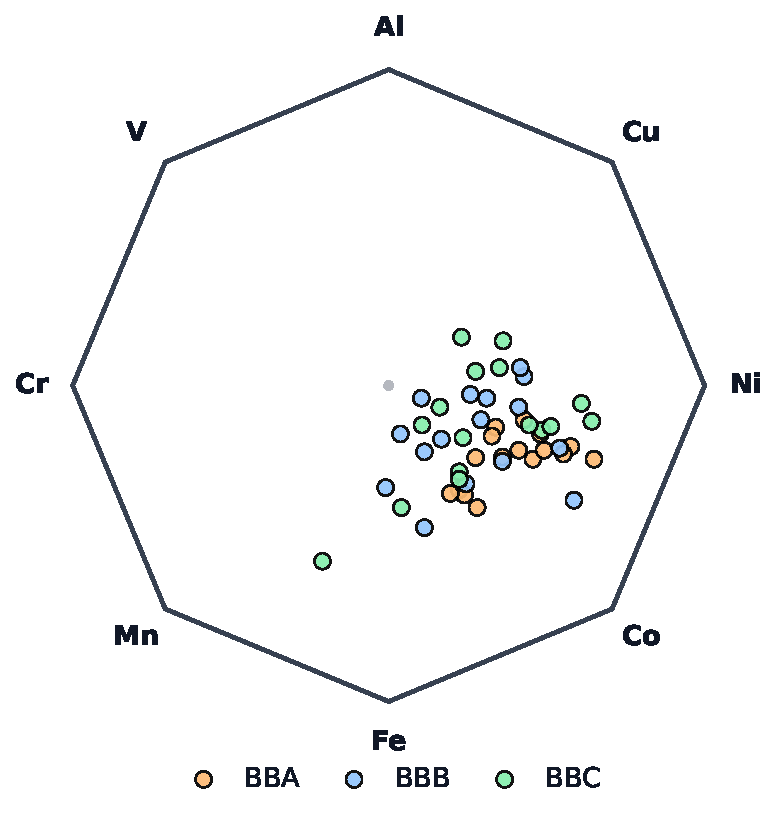
\includegraphics[width=0.95\columnwidth]{Figures/alloy_affine_projection.pdf}
    \caption{Affine projection of the target chemistries of all 48 alloys synthesized in this study onto a regular octagon representing the 8-element composition space (Al--V--Cr--Mn--Fe--Co--Ni--Cu). Each point is the affine-coordinate projection of one alloy composition and is colored by design iteration.} %The affine and UMAP projections (\autoref{fig:umap_alloyspace}) serve the same purpose; the affine projection was adopted here as a linear, interpretable alternative.
    \label{fig:alloy_affine_projection}
\end{figure} 

\autoref{fig:Phase_Analysis}(a--c) presents the diffraction patterns across all three iterations: the majority of alloys show single-phase FCC reflections at (111), (200), and (220), consistent with the CALPHAD-based design targets. Secondary intermetallic sigma ($P4_{2}/mnm$) phase was detected in a subset of alloys from iterations BBB and BBC.

\begin{figure*}[t]
    \centering
    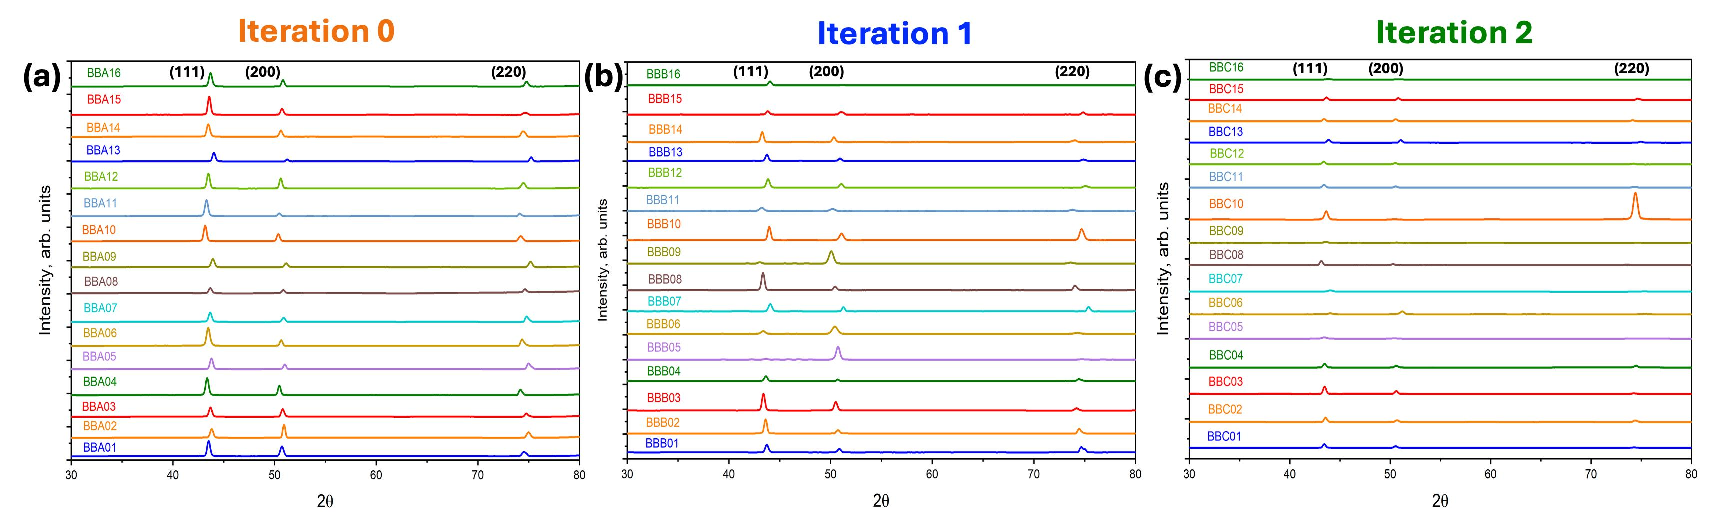
\includegraphics[width=0.95\textwidth]{Figures/phase_analysis_C2.pdf}
    \caption{X-ray diffraction (XRD) patterns for all alloys across 3 iterations (a--c), showing FCC spectral peaks at (111), (200), and (220) planar reflections. Alloys with secondary sigma phase are indicated.}
    \label{fig:Phase_Analysis}
\end{figure*}

Sigma phase appeared preferentially in alloys with combined V + Cr content $\geq$ 20~at.\%, although several alloys with high V + Cr (BBA09, BBB01, BBB03, BBC02, BBC04) remained single-phase FCC. These exceptions had Ni content of 36~at.\% or higher, consistent with increased valence electron concentration (VEC) destabilizing the sigma phase. We note that this compositional dependence---sigma formation correlating with V + Cr and suppressed by Ni---directly informed the GPC feasibility classifier training data.

The sigma-phase failures in BBB triggered a transition from the TCHEA6 to TCHEA7 database and the addition of a 950$^\circ$C FCC stability constraint (Section~2.1.2). Comparing TCHEA7 predictions with experimental XRD results for iterations BBA and BBB revealed five false positives (secondary phases predicted but not observed) and two false negatives (FCC predicted but sigma observed) at 700$^\circ$C, and one false positive and four false negatives at 950$^\circ$C. False negatives are the more consequential error: they lead to failed experiments (i.e., budget spent without usable objective data). These prediction discrepancies quantify the CALPHAD model uncertainty that the GPC feasibility classifier is designed to absorb.

\autoref{fig:BSE_SEM}(a--c) presents BSE-SEM images of three representative alloy compositions (one per iteration), showing fully recrystallized, equiaxed FCC grain structures with annealing twins. No significant porosity or macrosegregation was observed. The corresponding EBSD inverse pole figure (IPF) maps (\autoref{fig:BSE_SEM}(d--f)) confirm the absence of textural anisotropy, indicating that recrystallization reset the deformation-induced orientation bias from cold rolling. 
Grain size distributions (\autoref{fig:BSE_SEM}(g--i)) show average grain sizes between 10~$\mu$m and 35~$\mu$m, with compositionally complex alloys (7--8 elements) showing finer grains and narrower distributions, consistent with sluggish diffusion in concentrated solid solutions.

\begin{figure*}[t]
    \centering
    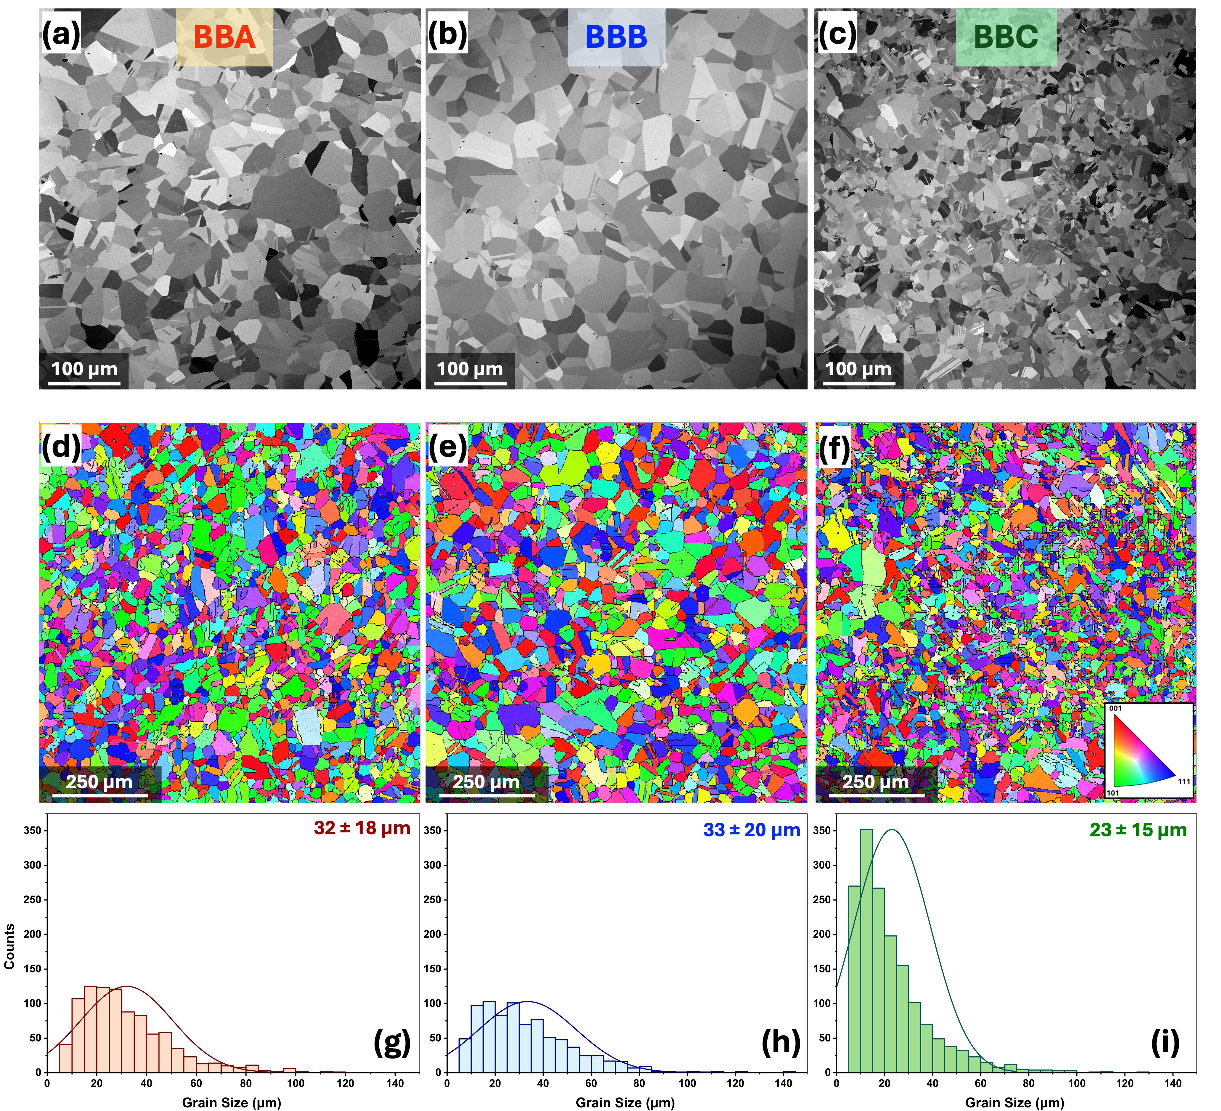
\includegraphics[width=0.7\textwidth]{Figures/BSE_SEM_v3.pdf}
    \caption{Microstructure of representative FCC alloy compositions across 3 iterations. (a--c) SEM-BSE micrographs showing fully recrystallized equiaxed FCC grains with annealing twins. (d--f) Corresponding EBSD IPF maps confirming random crystallographic texture. (g--i) Grain size histograms with descriptive statistics. Mean grain sizes range from $\sim$10~$\mu$m to 35~$\mu$m.}
    \label{fig:BSE_SEM}
\end{figure*}

Alloys confirmed as single-phase FCC proceeded to full mechanical characterization, and we used their objective measurements to train the GP surrogates. Alloys containing sigma phase were classified as infeasible for the purposes of Bayesian optimization: their phase outcome was used to retrain the GPC feasibility classifier, but their objective measurements (when obtainable) were not included in surrogate model training. Several sigma-bearing alloys (BBC03, BBB13, BBC08, BBC14) retained sufficient FCC matrix to yield tensile specimens and were mechanically tested for scientific characterization, but their properties were excluded from the BO loop. Alloys that failed during processing (BBC05--07, BBC09--10, BBC16, BBA04) produced no specimens and contributed only their infeasible label to the GPC. \autoref{table_bba}, \autoref{table_bbb}, and \autoref{table_bbc} list the target and measured compositions (EDS) alongside XRD phase verification for all three iterations. Candidates that violated project constraints (manufacturing failures or secondary phases) are highlighted in red.

\begin{table*}[t]
\caption{Composition and phase analysis of BBA (Iteration 0) alloys}
\label{table_bba}
\centering
\scriptsize
\resizebox{\textwidth}{!}{
\begin{tblr}{
    hlines,
    hline{3,21} = {2pt},
    rowsep=1pt,
    colspec = {
        |X[1.2, c]
        |[2pt]X[0.7, c]|X[0.7, c]|X[0.7, c]|X[0.7, c]|X[0.7, c]|X[0.7, c]|X[0.7, c]|X[0.7, c]
        |[2pt]X[0.7, c]|X[0.7, c]|X[0.7, c]|X[0.7, c]|X[0.7, c]|X[0.7, c]|X[0.7, c]|X[0.7, c]
        |[2pt]X[2.0, c]
        |X[2.0, c]|
        },
    colsep=0pt,
    }
    \SetCell[r=2,c=1]{c}\textbf{\makecell{Alloy\\Name}}
    & \SetCell[c=8]{c} \textbf{Target Atomic \%}
    &&&&&&&& \SetCell[c=8]{c} \textbf{EDS Measured Atomic \%}
    &&&&&&&& \SetCell[r=2,c=1]{c}\textbf{XRD Phase} \\
    & Al & Co & Cr & Cu & Fe & Mn & Ni & V
    & Al & Co & Cr & Cu & Fe & Mn & Ni & V \\
    BBA01 & 4 & 8 & 4 & 4 & 16 & 12 & 48 & 4 & 4.1 & 8.2 & 4.2 & 4.2 & 16.1 & 12.2 & 47.0 & 4.1 & FCC \\
    BBA02 & 4 & 16 & \SetCell{gray!20}0 & 4 & 12 & 8 & 52 & 4 & 4.2 & 15.0 & \SetCell{gray!20}0.0 & 4.2 & 12.2 & 8.2 & 52.2 & 4.1 & FCC \\
    BBA03 & 4 & 12 & 8 & 4 & 16 & 8 & 48 & \SetCell{gray!20}0 & 4.3 & 12.1 & 8.2 & 4.2 & 16.1 & 8.2 & 47.0 & \SetCell{gray!20}0.0 & FCC \\
    \SetCell{red!20}\textbf{BBA04} & \SetCell{gray!20}0 & 12 & 8 & 4 & 16 & 20 & 36 & 4 & $\cdot$ & $\cdot$ & $\cdot$ & $\cdot$ & $\cdot$ & $\cdot$ & $\cdot$ & $\cdot$ & \SetCell{red!20}\textbf{---} \\
    BBA05 & 4 & 12 & 8 & \SetCell{gray!20}0 & 8 & 8 & 56 & 4 & 4.1 & 12.2 & 8.2 & \SetCell{gray!20}0.0 & 8.2 & 8.0 & 55.2 & 4.1 & FCC \\
    BBA06 & 4 & \SetCell{gray!20}0 & 8 & 4 & 24 & 12 & 44 & 4 & 4.2 & \SetCell{gray!20}0.0 & 8.3 & 4.1 & 24.0 & 11.9 & 43.4 & 4.1 & FCC \\
    BBA07 & 4 & 12 & \SetCell{gray!20}0 & \SetCell{gray!20}0 & 16 & 8 & 52 & 8 & 5.0 & 12.3 & \SetCell{gray!20}0.0 & \SetCell{gray!20}0.0 & 16.2 & 7.9 & 50.5 & 8.1 & FCC \\
    BBA08 & \SetCell{gray!20}0 & 24 & 8 & \SetCell{gray!20}0 & 12 & 16 & 32 & 8 & \SetCell{gray!20}0.0 & 22.9 & 8.1 & \SetCell{gray!20}0.0 & 12.2 & 16.0 & 32.7 & 8.1 & FCC \\
    BBA09 & 4 & 16 & 8 & \SetCell{gray!20}0 & 12 & \SetCell{gray!20}0 & 48 & 12 & 4.9 & 16.1 & 8.2 & \SetCell{gray!20}0.0 & 12.0 & \SetCell{gray!20}0.0 & 46.6 & 12.1 & FCC \\
    BBA10 & 4 & \SetCell{gray!20}0 & 4 & \SetCell{gray!20}0 & 20 & 8 & 52 & 12 & 4.4 & \SetCell{gray!20}0.0 & 4.2 & \SetCell{gray!20}0.0 & 20.2 & 8.0 & 51.0 & 12.2 & FCC \\
    BBA11 & \SetCell{gray!20}0 & 16 & \SetCell{gray!20}0 & 4 & 20 & 20 & 28 & 12 & \SetCell{gray!20}0.0 & 16.1 & \SetCell{gray!20}0.0 & 4.0 & 20.1 & 20.3 & 27.4 & 12.0 & FCC \\
    BBA12 & \SetCell{gray!20}0 & \SetCell{gray!20}0 & 8 & 4 & 16 & 12 & 52 & 8 & \SetCell{gray!20}0.0 & \SetCell{gray!20}0.0 & 8.3 & 4.1 & 16.1 & 12.3 & 51.2 & 8.0 & FCC \\
    BBA13 & 4 & 20 & 4 & 4 & 16 & \SetCell{gray!20}0 & 52 & \SetCell{gray!20}0 & 4.0 & 20.4 & 4.1 & 4.2 & 16.3 & \SetCell{gray!20}0.0 & 51.0 & \SetCell{gray!20}0.0 & FCC \\
    BBA14 & \SetCell{gray!20}0 & 16 & 8 & 4 & 16 & 20 & 36 & \SetCell{gray!20}0 & \SetCell{gray!20}0.0 & 16.1 & 8.2 & 4.0 & 16.0 & 20.3 & 35.3 & \SetCell{gray!20}0.0 & FCC \\
    BBA15 & \SetCell{gray!20}0 & 20 & 8 & 4 & \SetCell{gray!20}0 & 20 & 44 & 4 & \SetCell{gray!20}0.0 & 19.9 & 8.2 & 4.2 & \SetCell{gray!20}0.0 & 20.5 & 43.2 & 4.0 & FCC \\
    BBA16 & 4 & 12 & \SetCell{gray!20}0 & 12 & 20 & 8 & 44 & \SetCell{gray!20}0 & 4.1 & 12.3 & \SetCell{gray!20}0.0 & 11.8 & 20.4 & 8.1 & 43.2 & \SetCell{gray!20}0.0 & FCC \\
\end{tblr}
}
\end{table*}

\begin{table*}[t]
\caption{Composition and phase analysis of BBB (Iteration 1) alloys}
\label{table_bbb}
\centering
\scriptsize
\resizebox{\textwidth}{!}{
\begin{tblr}{
    hlines,
    hline{3,17} = {2pt},
    rowsep=1pt,
    colspec = {
        |X[1.2, c]
        |[2pt]X[0.7, c]|X[0.7, c]|X[0.7, c]|X[0.7, c]|X[0.7, c]|X[0.7, c]|X[0.7, c]|X[0.7, c]
        |[2pt]X[0.7, c]|X[0.7, c]|X[0.7, c]|X[0.7, c]|X[0.7, c]|X[0.7, c]|X[0.7, c]|X[0.7, c]
        |[2pt]X[2.0, c]
        |X[2.0, c]|
        },
    colsep=0pt,
    }
    \SetCell[r=2,c=1]{c}\textbf{\makecell{Alloy\\Name}}
    & \SetCell[c=8]{c} \textbf{Target Atomic \%}
    &&&&&&&& \SetCell[c=8]{c} \textbf{EDS Measured Atomic \%}
    &&&&&&&& \SetCell[r=2,c=1]{c}\textbf{XRD Phase} \\
    & Al & Co & Cr & Cu & Fe & Mn & Ni & V
    & Al & Co & Cr & Cu & Fe & Mn & Ni & V \\
    BBB01 & \SetCell{gray!20}0 & 24 & 4 & \SetCell{gray!20}0 & 8 & 4 & 36 & 24 & \SetCell{gray!20}0.0 & 20.5 & 4.2 & \SetCell{gray!20}0.0 & 8.1 & 4.0 & 38.9 & 24.4 & FCC \\
    BBB02 & 4 & 32 & 8 & 4 & 4 & 20 & 24 & 4 & 4.2 & 30.4 & 8.2 & 4.1 & 4.1 & 20.1 & 24.7 & 4.1 & FCC \\
    BBB03 & 4 & \SetCell{gray!20}0 & 12 & 4 & 4 & 16 & 52 & 8 & 4.1 & $\cdot$ & 12.3 & 4.1 & 4.1 & 16.1 & 51.2 & 8.2 & FCC \\
    BBB04 & 4 & 12 & 4 & \SetCell{gray!20}0 & 28 & \SetCell{gray!20}0 & 40 & 12 & 4.0 & 11.1 & 4.1 & \SetCell{gray!20}0.0 & 28.0 & \SetCell{gray!20}0.0 & 40.8 & 12.0 & FCC \\
    \SetCell{red!20}\textbf{BBB05} & \SetCell{gray!20}0 & 44 & 12 & \SetCell{gray!20}0 & 4 & 4 & 12 & 24 & $\cdot$ & $\cdot$ & $\cdot$ & $\cdot$ & $\cdot$ & $\cdot$ & $\cdot$ & $\cdot$ & \SetCell{red!20}\textbf{$\mathbf{FCC+\sigma}$} \\
    \SetCell{red!20}\textbf{BBB06} & \SetCell{gray!20}0 & 16 & 20 & \SetCell{gray!20}0 & 4 & 4 & 36 & 20 & $\cdot$ & $\cdot$ & $\cdot$ & $\cdot$ & $\cdot$ & $\cdot$ & $\cdot$ & $\cdot$ & \SetCell{red!20}\textbf{$\mathbf{FCC+\sigma}$} \\
    BBB07 & 4 & 40 & \SetCell{gray!20}0 & \SetCell{gray!20}0 & 12 & 4 & 36 & 4 & 4.0 & 39.1 & \SetCell{gray!20}0.0 & \SetCell{gray!20}0.0 & 12.3 & 3.9 & 36.7 & 4.0 & FCC \\
    BBB08 & 4 & 8 & 12 & 4 & 4 & 24 & 40 & 4 & 3.8 & 8.0 & 12.3 & 4.2 & 4.1 & 24.0 & 39.4 & 4.1 & FCC \\
    \SetCell{red!20}\textbf{BBB09} & \SetCell{gray!20}0 & 4 & 8 & \SetCell{gray!20}0 & 4 & 28 & 40 & 16 & $\cdot$ & $\cdot$ & $\cdot$ & $\cdot$ & $\cdot$ & $\cdot$ & $\cdot$ & $\cdot$ & \SetCell{red!20}\textbf{$\mathbf{FCC+\sigma}$} \\
    BBB10 & 4 & \SetCell{gray!20}0 & 4 & 4 & 8 & 16 & 52 & 12 & $\cdot$ & $\cdot$ & $\cdot$ & $\cdot$ & $\cdot$ & $\cdot$ & $\cdot$ & $\cdot$ & FCC \\
    \SetCell{red!20}\textbf{BBB11} & \SetCell{gray!20}0 & 24 & 4 & \SetCell{gray!20}0 & 4 & 32 & 20 & 16 & $\cdot$ & $\cdot$ & $\cdot$ & $\cdot$ & $\cdot$ & $\cdot$ & $\cdot$ & $\cdot$ & \SetCell{red!20}\textbf{$\mathbf{FCC+\sigma}$} \\
    BBB12 & \SetCell{gray!20}0 & 20 & 4 & \SetCell{gray!20}0 & 4 & 4 & 48 & 20 & \SetCell{gray!20}0.0 & 20.2 & 4.2 & \SetCell{gray!20}0.0 & 4.1 & 4.0 & 47.1 & 20.4 & FCC \\
    \SetCell{red!20}\textbf{BBB13} & \SetCell{gray!20}0 & 40 & 4 & \SetCell{gray!20}0 & 28 & 4 & 4 & 20 & 0.0 & 39.7 & 4.2 & 0.0 & 27.9 & 3.9 & 4.2 & 20.1 & \SetCell{red!20}\textbf{$\mathbf{FCC+\sigma}$} \\
    BBB14 & 4 & \SetCell{gray!20}0 & 12 & 16 & 4 & 12 & 52 & \SetCell{gray!20}0 & 4.4 & \SetCell{gray!20}0.0 & 12.1 & 15.7 & 4.1 & 12.4 & 51.3 & \SetCell{gray!20}0.0 & FCC \\
    BBB15 & 4 & \SetCell{gray!20}0 & 8 & 24 & 4 & 16 & 44 & \SetCell{gray!20}0 & 4.3 & \SetCell{gray!20}0.0 & 8.3 & 23.5 & 4.1 & 16.2 & 43.7 & \SetCell{gray!20}0.0 & FCC \\
    BBB16 & 4 & 36 & \SetCell{gray!20}0 & \SetCell{gray!20}0 & 4 & 4 & 40 & 12 & $\cdot$ & $\cdot$ & $\cdot$ & $\cdot$ & $\cdot$ & $\cdot$ & $\cdot$ & $\cdot$ & FCC \\
\end{tblr}
}
\end{table*}

\begin{table*}[t]
\caption{Composition and phase analysis of BBC (Iteration 2) alloys}
\label{table_bbc}
\centering
\scriptsize
\resizebox{\textwidth}{!}{
\begin{tblr}{
    hlines,
    hline{3,17} = {2pt},
    rowsep=1pt,
    colspec = {
        |X[1.2, c]
        |[2pt]X[0.7, c]|X[0.7, c]|X[0.7, c]|X[0.7, c]|X[0.7, c]|X[0.7, c]|X[0.7, c]|X[0.7, c]
        |[2pt]X[0.7, c]|X[0.7, c]|X[0.7, c]|X[0.7, c]|X[0.7, c]|X[0.7, c]|X[0.7, c]|X[0.7, c]
        |[2pt]X[2.0, c]
        |X[2.0, c]|
        },
    colsep=0pt,
    }
    \SetCell[r=2,c=1]{c}\textbf{\makecell{Alloy\\Name}}
    & \SetCell[c=8]{c} \textbf{Target Atomic \%}
    &&&&&&&& \SetCell[c=8]{c} \textbf{EDS Measured Atomic \%}
    &&&&&&&& \SetCell[r=2,c=1]{c}\textbf{XRD Phase} \\
    & Al & Co & Cr & Cu & Fe & Mn & Ni & V
    & Al & Co & Cr & Cu & Fe & Mn & Ni & V \\
    BBC01 & 4 & 12 & 4 & 4 & 20 & 16 & 32 & 8 & 4.0 & 12.2 & 4.2 & 4.0 & 20.1 & 16.0 & 31.4 & 8.2 & FCC \\
    BBC02 & 4 & 8 & \SetCell{gray!20}0 & \SetCell{gray!20}0 & 4 & 8 & 52 & 24 & 4.0 & 8.2 & \SetCell{gray!20}0.0 & \SetCell{gray!20}0.0 & 4.1 & 8.0 & 51.2 & 24.4 & FCC \\
    \SetCell{red!20}\textbf{BBC03} & 4 & 4 & 12 & \SetCell{gray!20}0 & \SetCell{gray!20}0 & 4 & 52 & 24 & 4.0 & 4.1 & 12.2 & \SetCell{gray!20}0.0 & \SetCell{gray!20}0.0 & 3.9 & 51.3 & 24.4 & \SetCell{red!20}\textbf{$\mathbf{FCC+\sigma}$} \\
    BBC04 & 4 & \SetCell{gray!20}0 & 4 & \SetCell{gray!20}0 & 4 & 4 & 60 & 24 & 4.0 & \SetCell{gray!20}0.0 & 4.2 & \SetCell{gray!20}0.0 & 4.1 & 4.0 & 59.3 & 24.5 & FCC \\
    \SetCell{red!20}\textbf{BBC05} & \SetCell{gray!20}0 & 24 & 8 & \SetCell{gray!20}0 & 16 & 40 & 4 & 8 & $\cdot$ & $\cdot$ & $\cdot$ & $\cdot$ & $\cdot$ & $\cdot$ & $\cdot$ & $\cdot$ & \SetCell{red!20}\textbf{---} \\
    \SetCell{red!20}\textbf{BBC06} & 4 & 28 & 4 & \SetCell{gray!20}0 & 4 & 4 & 44 & 12 & $\cdot$ & $\cdot$ & $\cdot$ & $\cdot$ & $\cdot$ & $\cdot$ & $\cdot$ & $\cdot$ & \SetCell{red!20}\textbf{---} \\
    \SetCell{red!20}\textbf{BBC07} & 4 & 32 & 4 & \SetCell{gray!20}0 & \SetCell{gray!20}0 & 4 & 44 & 12 & $\cdot$ & $\cdot$ & $\cdot$ & $\cdot$ & $\cdot$ & $\cdot$ & $\cdot$ & $\cdot$ & \SetCell{red!20}\textbf{---} \\
    \SetCell{red!20}\textbf{BBC08} & \SetCell{gray!20}0 & 8 & \SetCell{gray!20}0 & 4 & 4 & 28 & 36 & 20 & $\cdot$ & 8.1 & $\cdot$ & 4.1 & 4.2 & 28.1 & 35.7 & 19.9 & \SetCell{red!20}\textbf{$\mathbf{FCC+\sigma}$} \\
    \SetCell{red!20}\textbf{BBC09} & \SetCell{gray!20}0 & 36 & 4 & \SetCell{gray!20}0 & 16 & 16 & 8 & 20 & $\cdot$ & $\cdot$ & $\cdot$ & $\cdot$ & $\cdot$ & $\cdot$ & $\cdot$ & $\cdot$ & \SetCell{red!20}\textbf{---} \\
    \SetCell{red!20}\textbf{BBC10} & 4 & 4 & 16 & \SetCell{gray!20}0 & 8 & \SetCell{gray!20}0 & 52 & 16 & $\cdot$ & $\cdot$ & $\cdot$ & $\cdot$ & $\cdot$ & $\cdot$ & $\cdot$ & $\cdot$ & \SetCell{red!20}\textbf{---} \\
    BBC11 & 4 & 12 & 4 & 4 & 12 & 16 & 36 & 12 & 4.3 & 12.2 & 4.2 & 3.9 & 12.2 & 15.9 & 35.1 & 12.3 & FCC \\
    BBC12 & 4 & 4 & 4 & 8 & 28 & 16 & 32 & 4 & 4.1 & 4.3 & 4.2 & 7.8 & 28.0 & 16.1 & 31.3 & 4.1 & FCC \\
    BBC13 & 4 & 28 & \SetCell{gray!20}0 & 20 & 4 & 8 & 36 & \SetCell{gray!20}0 & 4.3 & 28.0 & $\cdot$ & 19.9 & 4.1 & 8.4 & 35.4 & $\cdot$ & FCC \\
    \SetCell{red!20}\textbf{BBC14} & \SetCell{gray!20}0 & 12 & 4 & \SetCell{gray!20}0 & 4 & 16 & 40 & 24 & $\cdot$ & 12.1 & 4.1 & $\cdot$ & 4.3 & 16.1 & 39.0 & 24.5 & \SetCell{red!20}\textbf{$\mathbf{FCC+\sigma}$} \\
    BBC15 & 4 & 16 & \SetCell{gray!20}0 & 20 & 4 & 12 & 44 & \SetCell{gray!20}0 & 4.4 & 16.2 & $\cdot$ & 19.7 & 4.2 & 12.3 & 43.3 & $\cdot$ & FCC \\
    \SetCell{red!20}\textbf{BBC16} & 4 & 28 & 4 & \SetCell{gray!20}0 & 8 & \SetCell{gray!20}0 & 40 & 16 & $\cdot$ & $\cdot$ & $\cdot$ & $\cdot$ & $\cdot$ & $\cdot$ & $\cdot$ & $\cdot$ & \SetCell{red!20}\textbf{---} \\
\end{tblr}
}
\end{table*}


\subsection{Mechanical Properties Across Iterations}

\subsubsection{Tensile Response}

\autoref{fig:true_stress_strain} presents the true stress--strain curves for all tested FCC alloys across the three iterations. True fracture stress increased progressively across successive iterations, with the majority of alloys surpassing 1~GPa in true tensile strength by iteration BBB. Ductility remained comparable across iterations, with the top-performing alloys sustaining strain at UTS in the range of 45--50\%. Enhanced strain hardening across iterations delayed the onset of strain localization, manifesting as high UTS/YS ratios. Compositions with UTS/YS $>$ 3.5 demonstrated superior strain hardening capacity, contributing to delayed failure under quasi-static loading. For context, Campaign~1 achieved UTS/YS ratios ranging from 1.38 to 2.93~\cite{hastings2025accelerated}. In Campaign~2, every successfully tested single-phase FCC alloy exceeded Campaign~1's maximum: the minimum UTS/YS was 3.07 (BBA07), the median was 3.79, and 9 alloys exceeded 4.0. 
We note that this wholesale improvement over Campaign~1 is not attributable to the optimizer alone. The GP surrogates in Campaign~2 were initialized with informative priors trained on Campaign~1 experimental data and the Varvenne--Luque--Curtin solid solution strengthening model (Section~2.6), giving the optimizer a physics-grounded starting point rather than a zero-mean prior. The design space was shaped by Campaign~1's experience: we expanded from 6 to 8 elements based on the observation that the 6-element space lacked sufficient compositional freedom to simultaneously maximize strength and ductility, and we replaced hardness with tensile-derived objectives (YS, UTS/YS, strain at UTS) based on the finding that hardness alone is an incomplete proxy for bulk mechanical response. The UTS/YS shift from 1.38--2.93 (Campaign~1) to 3.07--4.53 (Campaign~2) thus reflects the compounding effect of prior-informed surrogates, a better-chosen design space, and more directly relevant optimization objectives. Tabulated values of YS, UTS, and strain to failure for all tested alloys are provided in the \textbf{SI}.

\begin{figure}[H]
\centering
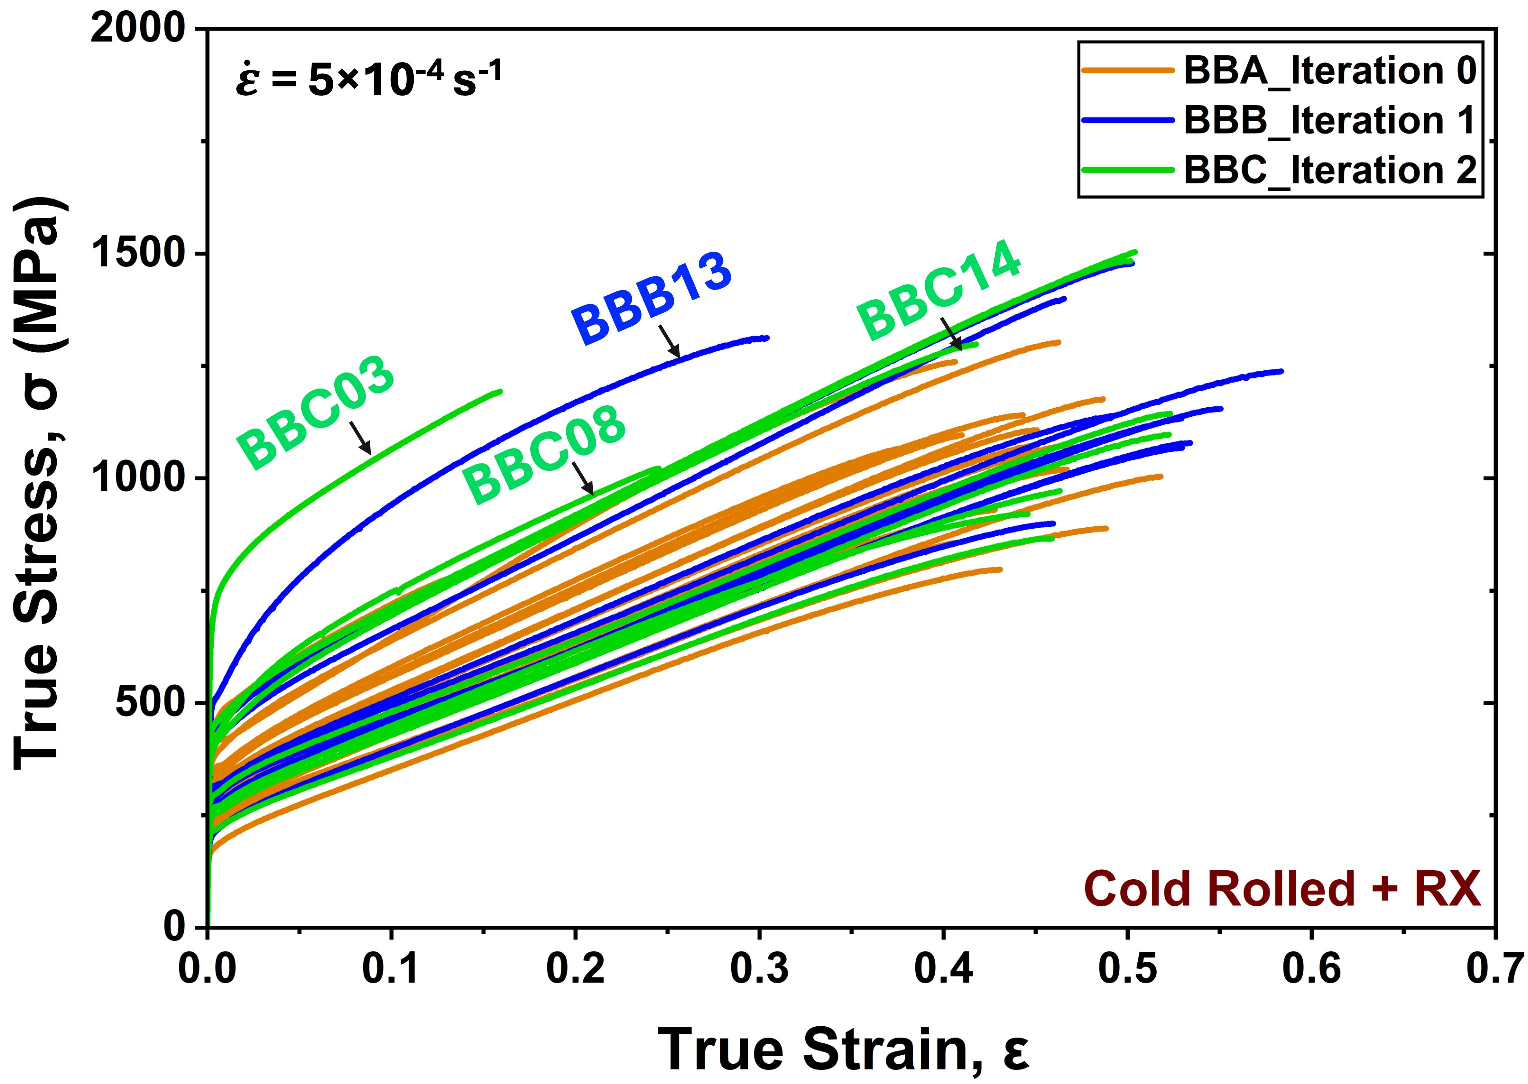
\includegraphics[width=0.9\columnwidth]{Figures/Tension_BBA_BBB_BBC.pdf}
\caption{Consolidated true stress--strain curves from ambient temperature quasistatic uniaxial tensile tests for all tested FCC alloys across 3 iterations. Alloys containing sigma phase are indicated by black arrows. RX refers to recrystallized alloys.}
\label{fig:true_stress_strain}
\end{figure}

\subsubsection{Dynamic Hardness and Rate Sensitivity}

Dynamic hardness consistently exceeded quasi-static hardness across all tested compositions (\autoref{fig:HSRNI1}), consistent with the higher strain rates associated with impact testing ($\sim 10^3$\,s$^{-1}$) relative to quasi-static indentation ($\sim 10^0$\,s$^{-1}$). Among single-phase FCC alloys, BBB12 showed the highest hardness. BBC03, which contained secondary sigma phase, showed the overall highest hardness.

\begin{figure*}[t]
    \centering
    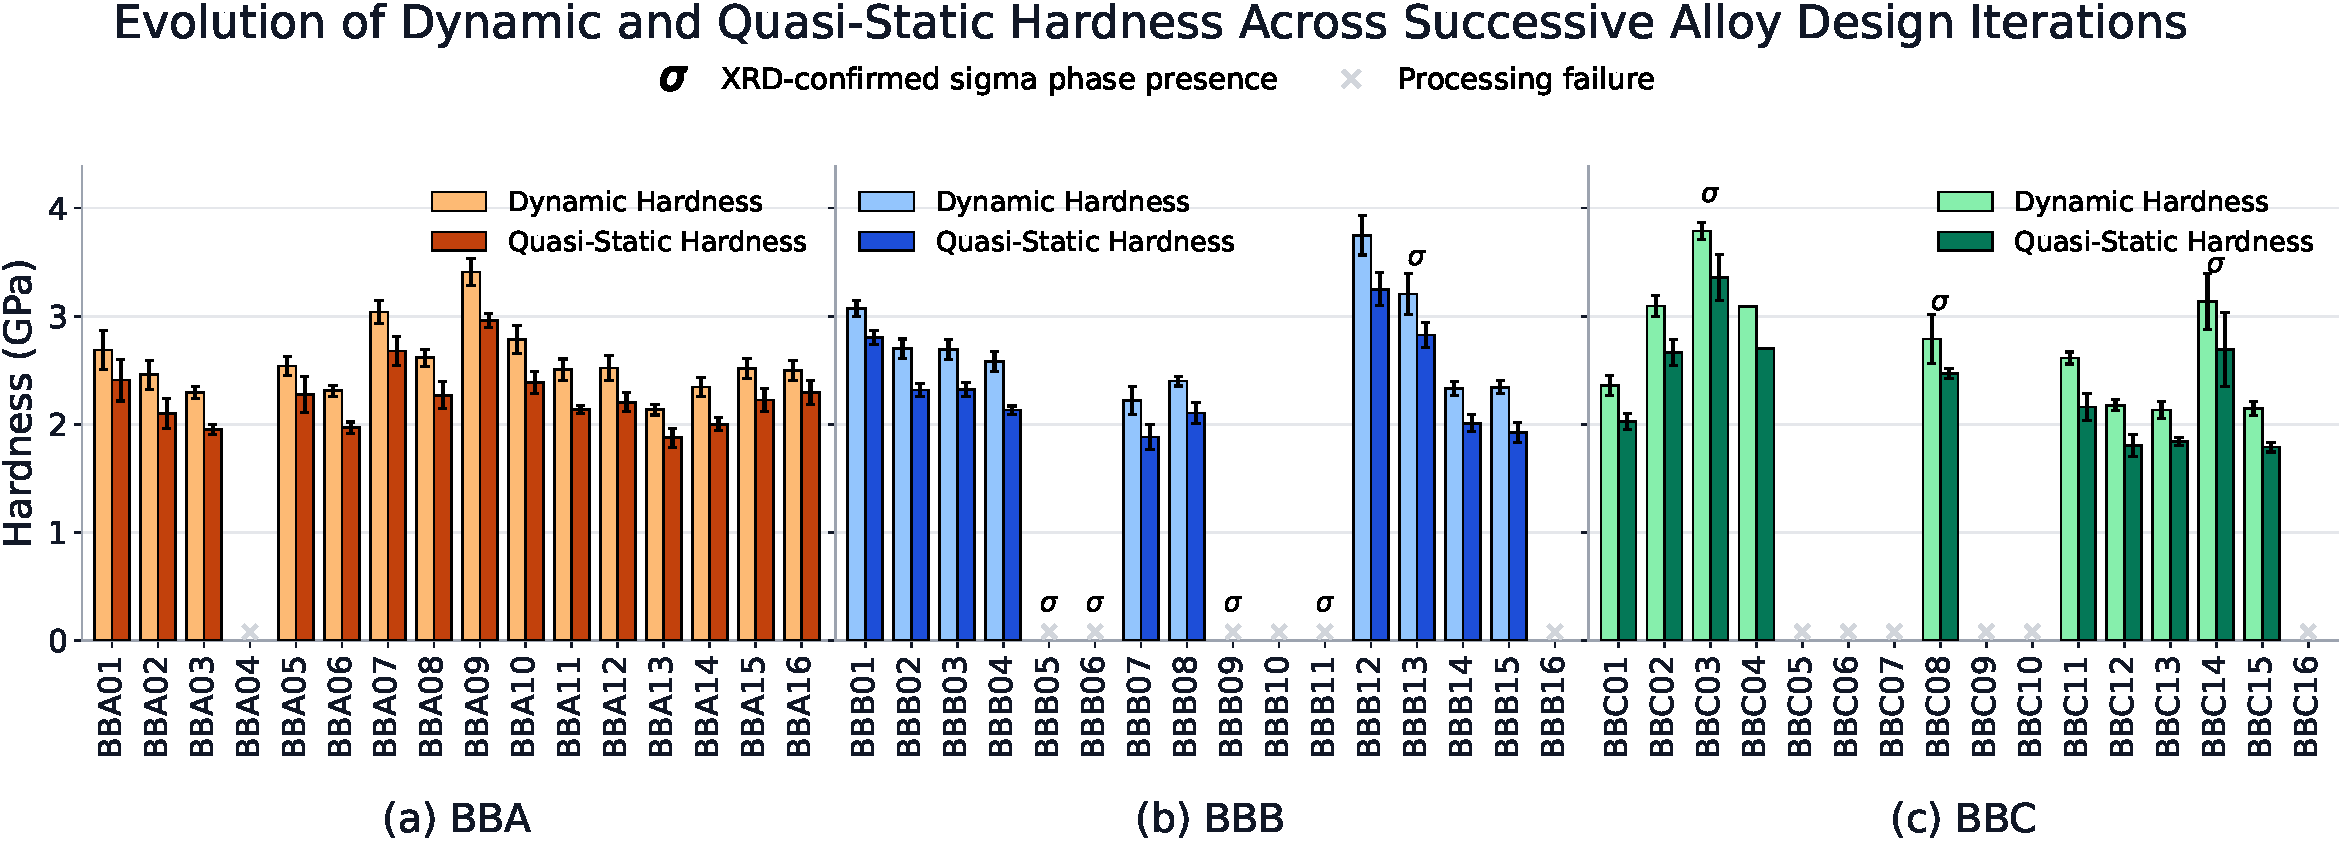
\includegraphics[width=\textwidth]{Figures/Hdyn_Hqs_1_02.pdf}
    \caption{Dynamic and quasistatic hardness values for all candidate alloys across iterations (a) BBA, (b) BBB, and (c) BBC. Bar colors are iteration-specific within each panel. Gray \texttimes{} markers denote processing failures with no hardness data, and $\sigma$ markers indicate alloys with XRD-confirmed sigma phase presence.}
    \label{fig:HSRNI1}
\end{figure*}

The dynamic-to-quasi-static hardness ratio, $H_{\text{DYN}}/H_{\text{QS}}$ (\autoref{fig:HSRNI2}), ranged from 1.09 to 1.22 across all samples, with no clear compositional trend. Error bars were computed via propagation of uncertainty from the standard deviations of both dynamic and quasi-static measurements. None of the tested compositions showed error bars overlapping with unity, confirming a measurable rate-dependent strengthening effect in every alloy.

\begin{figure*}[t]
    \centering
    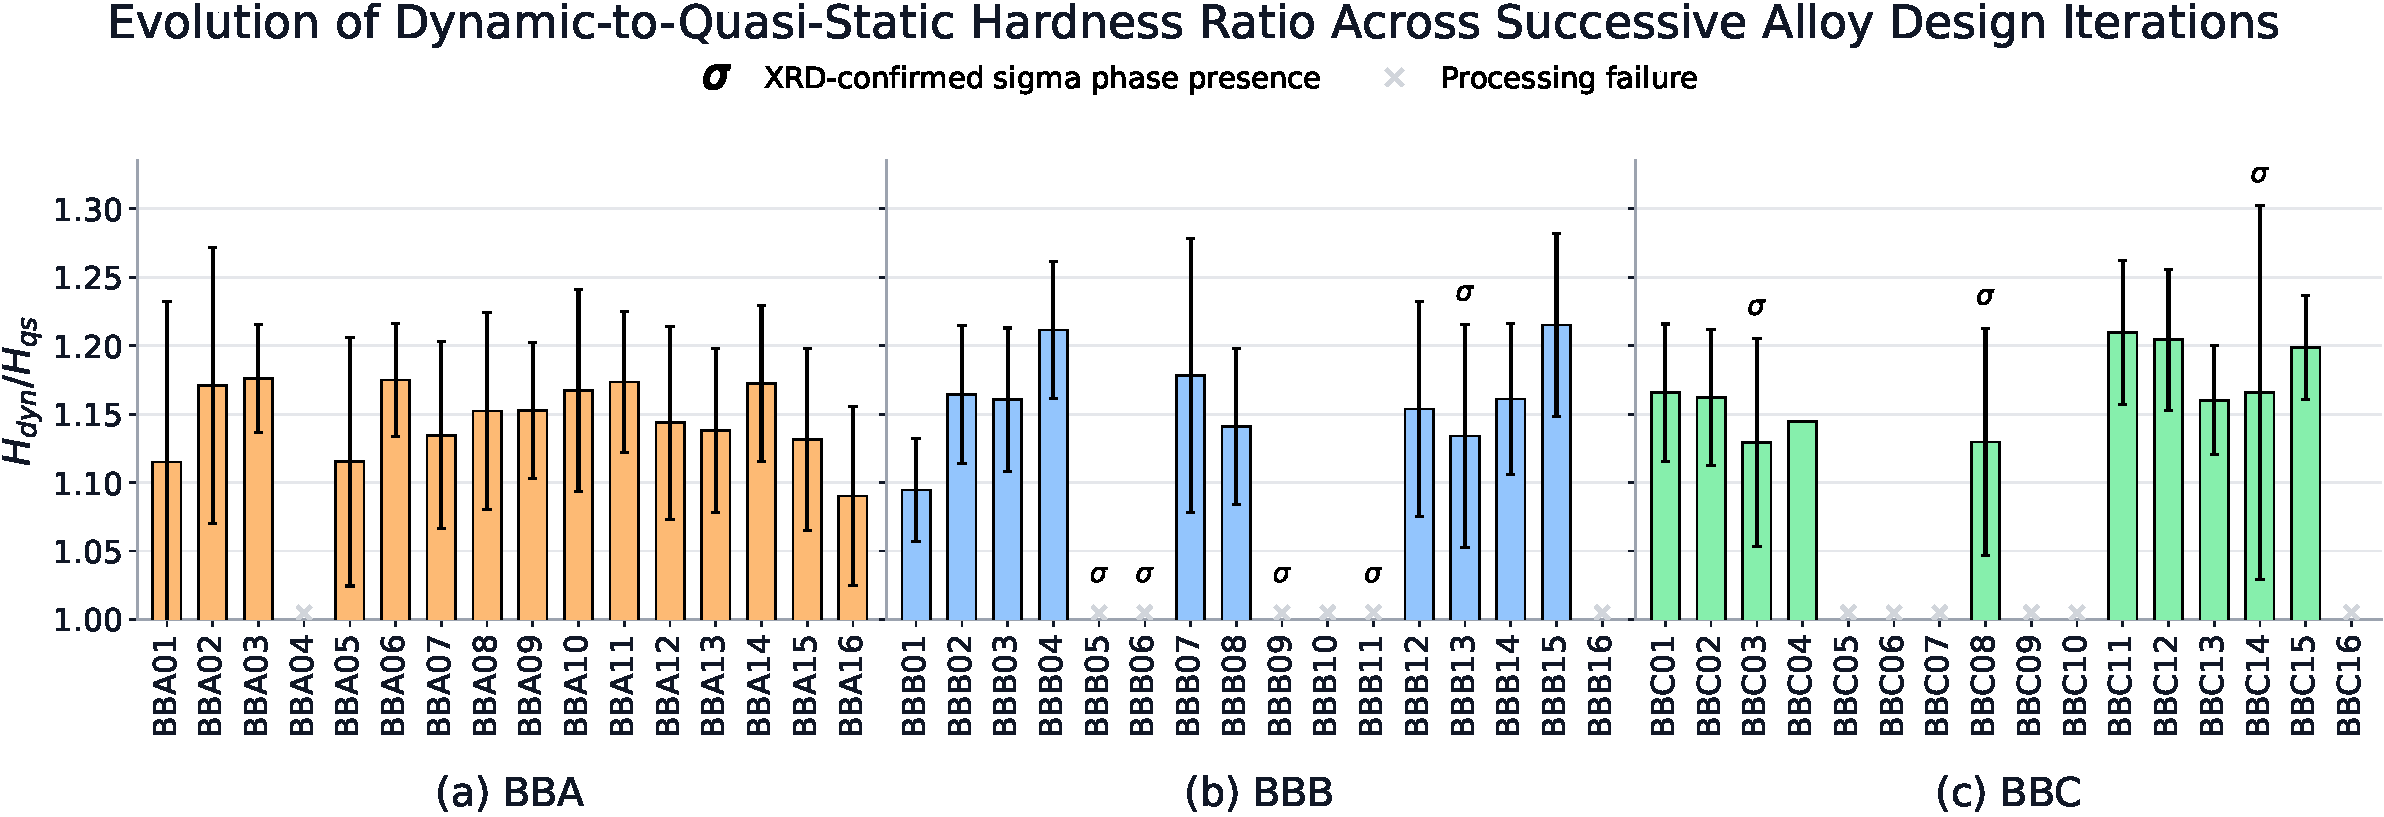
\includegraphics[width=\textwidth]{Figures/Dyn_QS_ratio_1.pdf}
    \caption{Dynamic-to-quasistatic hardness ratio ($H_{\mathrm{dyn}}/H_{\mathrm{qs}}$) for all candidate alloys across iterations (a) BBA, (b) BBB, and (c) BBC. Bar colors are iteration-specific within each panel. Gray \texttimes{} markers denote processing failures with no hardness-ratio data, and $\sigma$ markers indicate alloys with XRD-confirmed sigma phase presence.}
    \label{fig:HSRNI2}
\end{figure*}

The contact-depth-to-indentation-depth ratio ($h_c/h$) was close to 1 for most samples, indicating minimal pile-up or sink-in. BBC03 was an exception ($h_c/h$ up to 1.03), consistent with its sigma-phase-induced deformation behavior. The near-unity $h_c/h$ for single-phase FCC alloys supports the use of nominal hardness calculations, reducing the need for the time-consuming imaging and tracing steps required for precise contact area estimation.

\subsubsection{Depth of Penetration}

Simulated DoP values across all iterations ranged from 2.22 to 3.35~mm (tabulated in \textbf{SI}). The five best-performing alloys (lowest DoP)---BBC03, BBB13, BBC02, BBB01, and BBC04---were concentrated in iterations BBB and BBC, while the five worst-performing alloys (BBA13, BBA16, BBC15, BBA03, and BBB07) were predominantly from iteration BBA, with one (BBC15) from iteration BBC. This shift confirms that the Bayesian optimization loop progressively identified compositions with improved impact resistance. The 1.13~mm spread in DoP across the full dataset (3.35 $-$ 2.22~mm), though narrow in absolute terms, provided sufficient differentiation for the EHVI acquisition function to distinguish candidates.

\subsubsection{Property Evolution}

\autoref{fig:boxplot_properties} summarizes the statistical evolution of all measured properties across the three iterations. Median values for strength-related properties (YS, UTS, $H_\text{dyn}$, $H_\text{qs}$) increased from BBA to BBC while inter-quartile ranges narrowed, indicating convergence toward consistently high-performing compositions. Median DoP decreased across iterations, with the distribution tightening around lower penetration depths. Strain at UTS was maintained or improved despite the strength gains, confirming that the multi-objective framework avoided the classical strength--ductility trade-off.

\begin{figure*}[t]
    \centering
    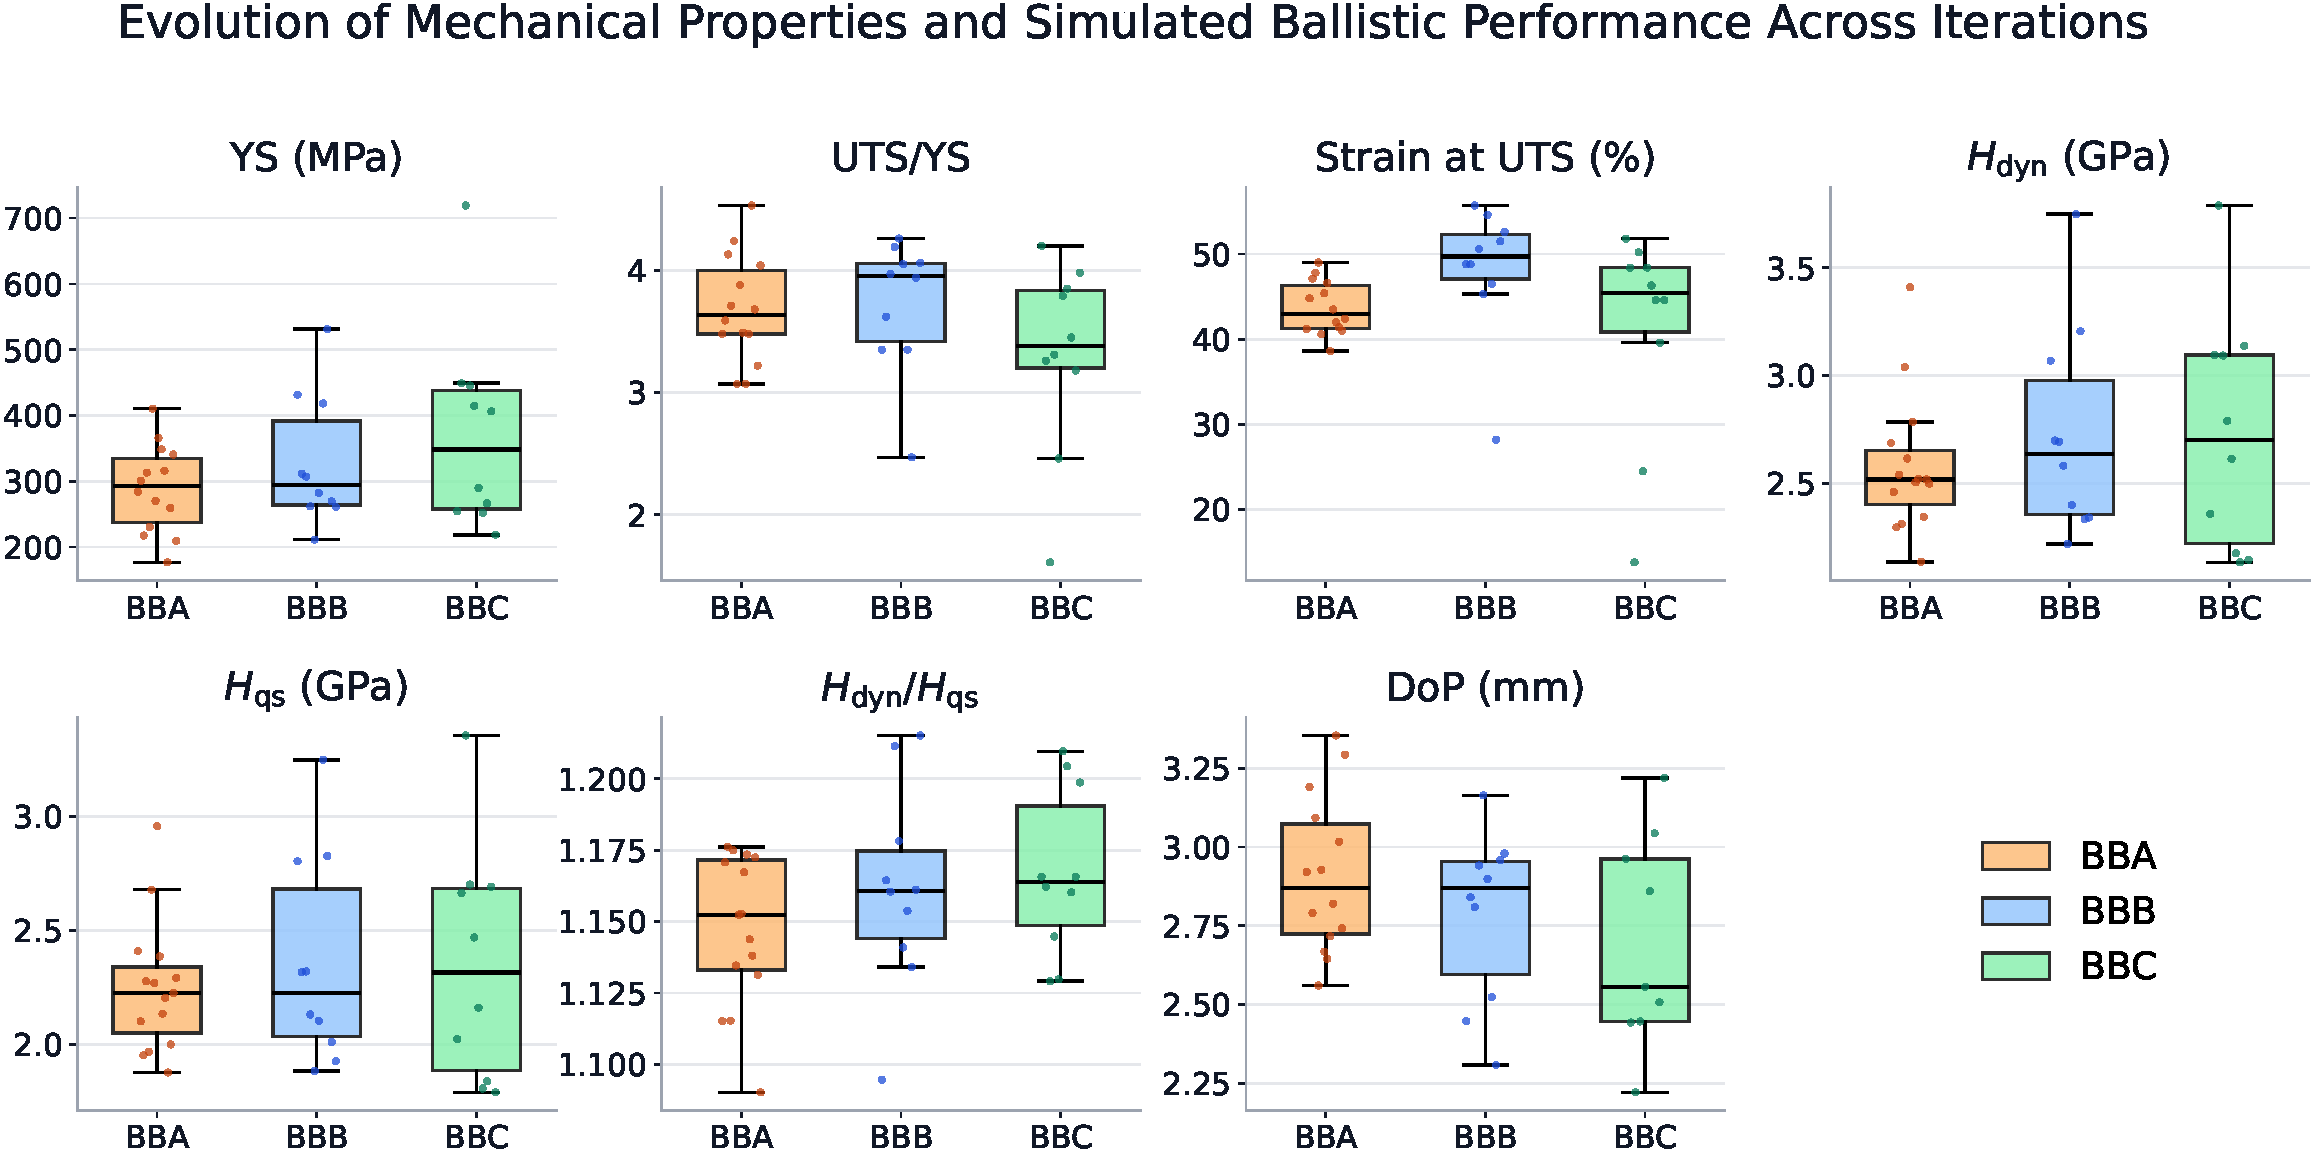
\includegraphics[width=0.9\textwidth]{Figures/box_plot.pdf}
    \caption{Evolution of mechanical properties and simulated ballistic performance across iterations. YS = yield strength, UTS = ultimate tensile strength, $H_{\mathrm{dyn}}$ = dynamic hardness, $H_{\mathrm{qs}}$ = quasistatic hardness, and DoP = simulated depth of penetration. Median strength metrics and $H_{\mathrm{dyn}}/H_{\mathrm{qs}}$ increase from BBA to BBC, while simulated depth of penetration decreases and strain at UTS is preserved.}
    \label{fig:boxplot_properties}
\end{figure*}

These improvements in median properties should be interpreted alongside a processing caveat. The optimization campaign treats composition as the sole design variable, but the measured properties also depend on thermomechanical processing history---specifically, the degree of cold work, recrystallization temperature, and resulting grain size. Several alloys that passed phase verification (single-phase FCC by XRD) showed anomalous tensile behavior: low ductility, premature failure, or high scatter between replicate specimens. Post-mortem analysis traced these anomalies to incomplete recrystallization or non-uniform grain size distributions rather than compositional effects. The consequence for the optimization loop is twofold. First, noisy property measurements reduce the signal-to-noise ratio available to the GP surrogates, slowing convergence. Second, alloys whose measured properties reflect processing defects rather than intrinsic compositional effects can mislead the acquisition function, directing the search toward or away from regions for the wrong reasons. Grain sizes in this campaign ranged from 10 to 35~$\mu$m (\autoref{fig:BSE_SEM}), and the more compositionally complex alloys (7--8 elements) generally showed finer, more uniform grains---consistent with sluggish diffusion reducing grain growth---and correspondingly lower property scatter. Standardizing the thermomechanical route to produce consistent, fully recrystallized microstructures across all compositions is a prerequisite for isolating compositional effects in future campaigns.

\subsection{Composition--Property Relationships}

\subsubsection{Correlation Structure and Feature Importance}

\autoref{fig:correlation_matrix} combines three complementary analyses: (a)~a Pearson correlation matrix quantifying linear relationships among elemental concentrations and mechanical responses, (b)~a SHAP beeswarm plot showing each element's importance and directional behavior in the predictive model, and (c)~a corrSHAP bar chart measuring the correlation between each element's compositional value and its SHAP contribution. SHAP values were computed from the gradient-boosted regression models trained independently on each of the five target objectives normalized per target, and pooled to give a single multi-objective view. The multi-objective corrSHAP (\autoref{fig:correlation_matrix}c) is the per-target Pearson correlation between feature value and SHAP value, averaged over the five target models. Positive values mean the element systematically raises the composite response across targets; cancellation across targets reflects a multi-objective trade-off.

\begin{figure*}[t]
    \centering
    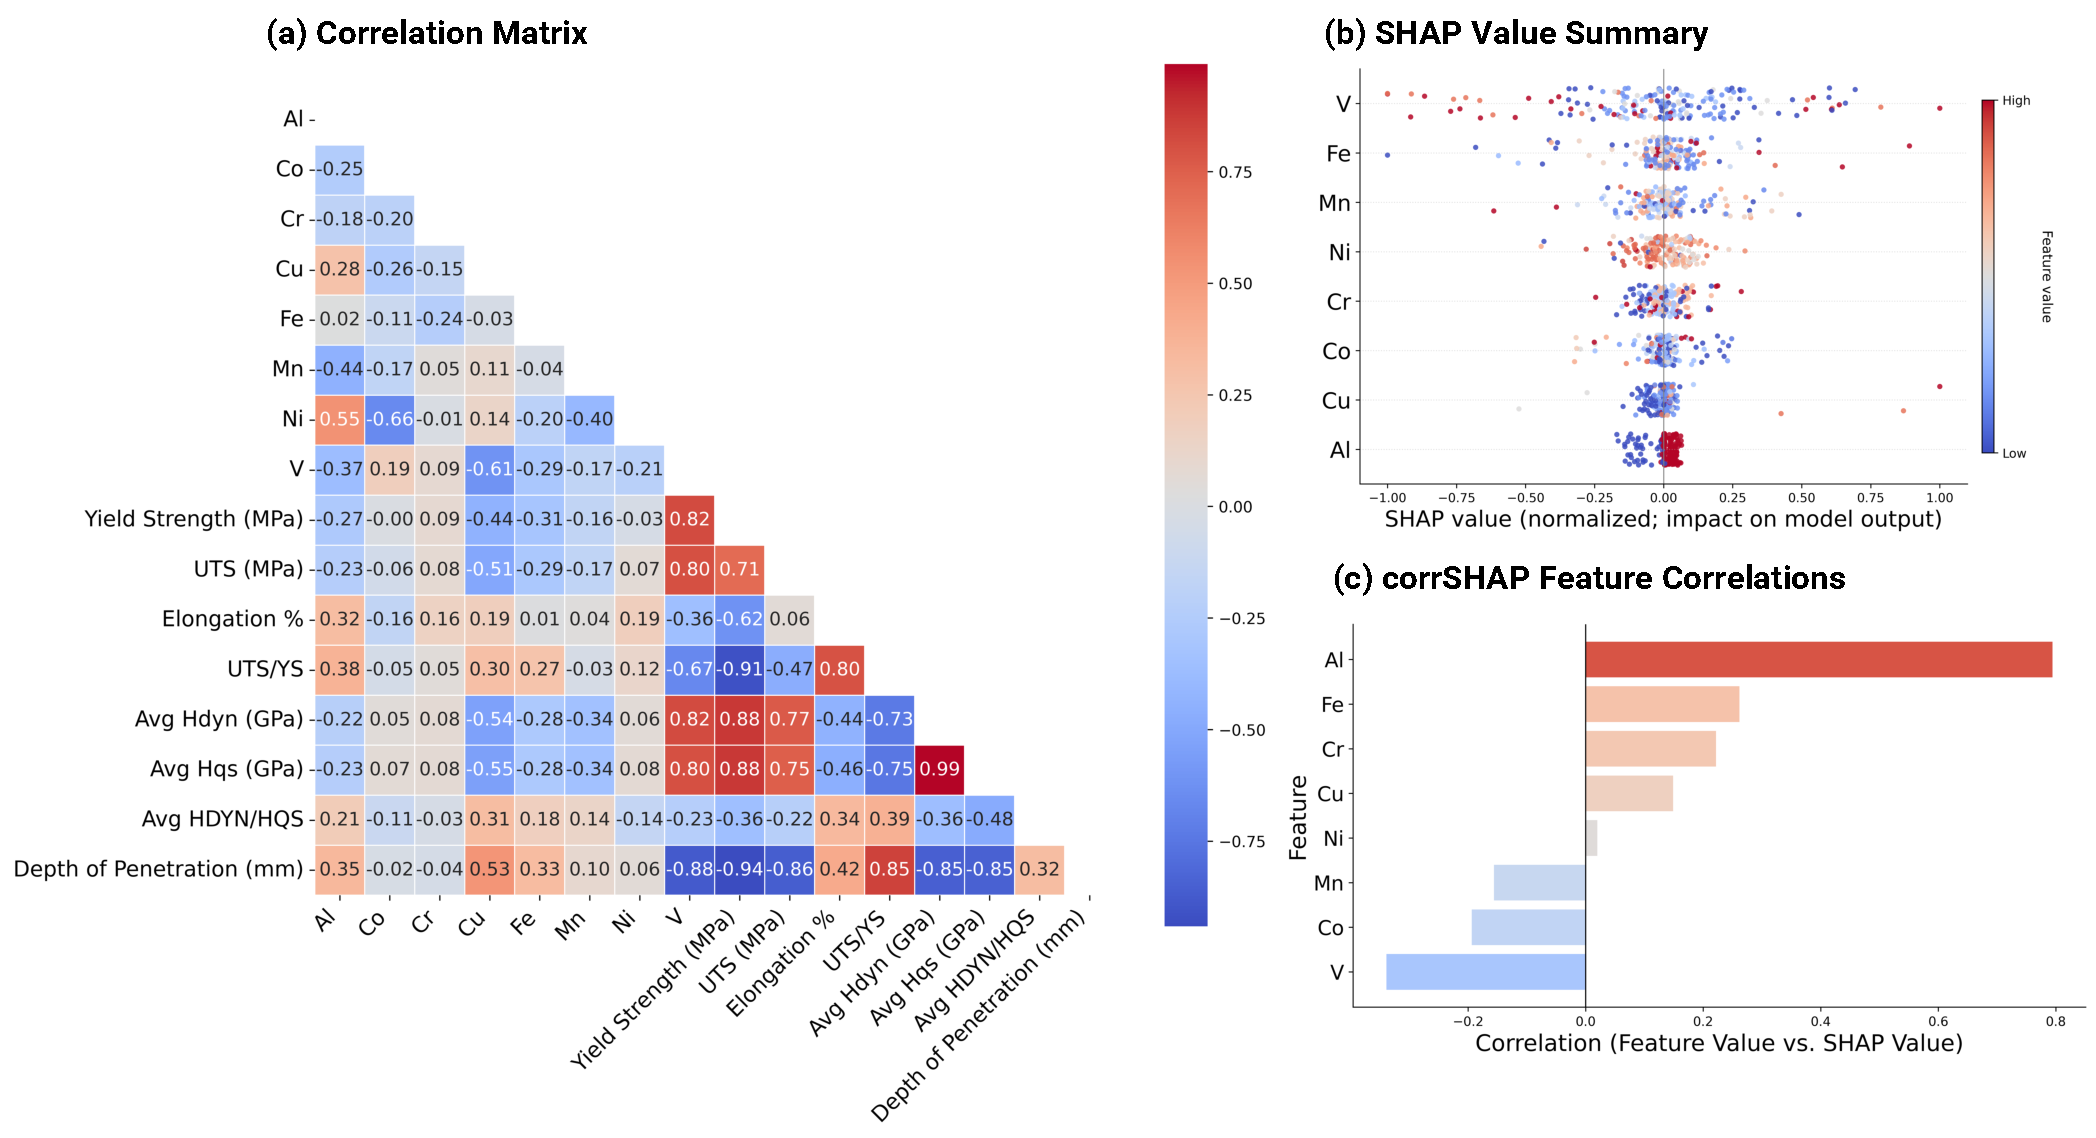
\includegraphics[width=1.0\textwidth]{Figures/correlation_matrix_v2.pdf}
    \caption{(a) Pearson correlation matrix among elemental concentrations, mechanical properties, and DoP. (b) SHAP beeswarm plot ranked by mean absolute SHAP value; dot color encodes feature value (red = high, blue = low). (c) corrSHAP bar chart showing the net directional influence of each element on the model output.}
    \label{fig:correlation_matrix}
\end{figure*}

Vanadium and copper define the primary compositional axis governing strength and penetration resistance. Vanadium shows strong positive correlations with YS ($r = 0.82$, $n = 37$), UTS ($r = 0.80$), and both hardness measures ($r \approx 0.81$), and a strong negative correlation with DoP ($r = -0.88$). Copper shows the opposite pattern: negative correlations with all strength metrics ($r = -0.44$ to $-0.55$) and positive correlation with DoP ($r = 0.53$). The V--Cu anticorrelation ($r = -0.61$) means the design space naturally partitions along this axis.

Among property--property relationships, YS and hardness are tightly coupled ($r = 0.88$), and the two hardness metrics are nearly identical ($r = 0.99$). UTS/YS is strongly anticorrelated with YS ($r = -0.91$) and positively correlated with elongation ($r = 0.80$), confirming that strain-hardening capacity accompanies ductility. DoP correlates almost perfectly (inversely) with YS ($r = -0.94$) and strongly with UTS ($r = -0.86$), indicating that penetration resistance in this alloy family is governed predominantly by strength.


SHAP and corrSHAP reflect the chosen multi-objective target and not single-property linear correlations. The SHAP results align with the linear correlations. Vanadium dominates mean $|\text{SHAP}|$, with normalized contributions spanning the full $[-1, +1]$ range; high-V points (red) at the positive tail and low-V (blue) at the
negative tail, matching V's positive correlations with strength metrics. Iron, manganese, and nickel follow; aluminum has the smallest mean $|\text{SHAP}|$ and clusters near zero. Mn and Ni dots show mixed colors at both positive and negative SHAP values, indicating interaction-mediated (non-monotonic) effects whose sign depends on the concentrations of other elements.
 
Aluminum has the strongest positive corrSHAP ($r \approx +0.78$), significantly higher than iron ($+0.27$), chromium ($+0.22$), and copper ($+0.15$) --- higher Al consistently pushes the composite up despite Al's modest $|\text{SHAP}|$ magnitude. This is consistent with aluminum's role as a solid solution strengthener in Ni-stabilized HEAs, where small additions of Al improve YS and UTS/YS without strongly penalizing ductility. Nickel is near zero ($r \approx 0$), confirming the sign-flipping, interaction-mediated behavior seen in SHAP beeswarm plot. The negative tail is vanadium ($-0.32$), cobalt ($-0.22$), and manganese ($-0.17$). Vanadium's negative multi-objective corrSHAP coexists with its strong positive correlations with strength because the composite also includes elongation and UTS/YS, with which V correlates $-0.36$ and $-0.67$, respectively. The ductility penalty associated with V (likely tied to its role in promoting sigma phase formation and reducing strain hardening capacity) dominates the strength benefit when all five objectives are weighted together. 


\subsubsection{Strength--Ductility Trade-off}

\autoref{fig:pair_plots} shows how the BBA (iteration~0), BBB (iteration~1), and BBC (iteration~2) alloys evolve through key strength--ductility property spaces, illustrating both improvement in feasible FCC alloys and the trade-off imposed by sigma phase formation.

\begin{figure*}[t]
    \centering
    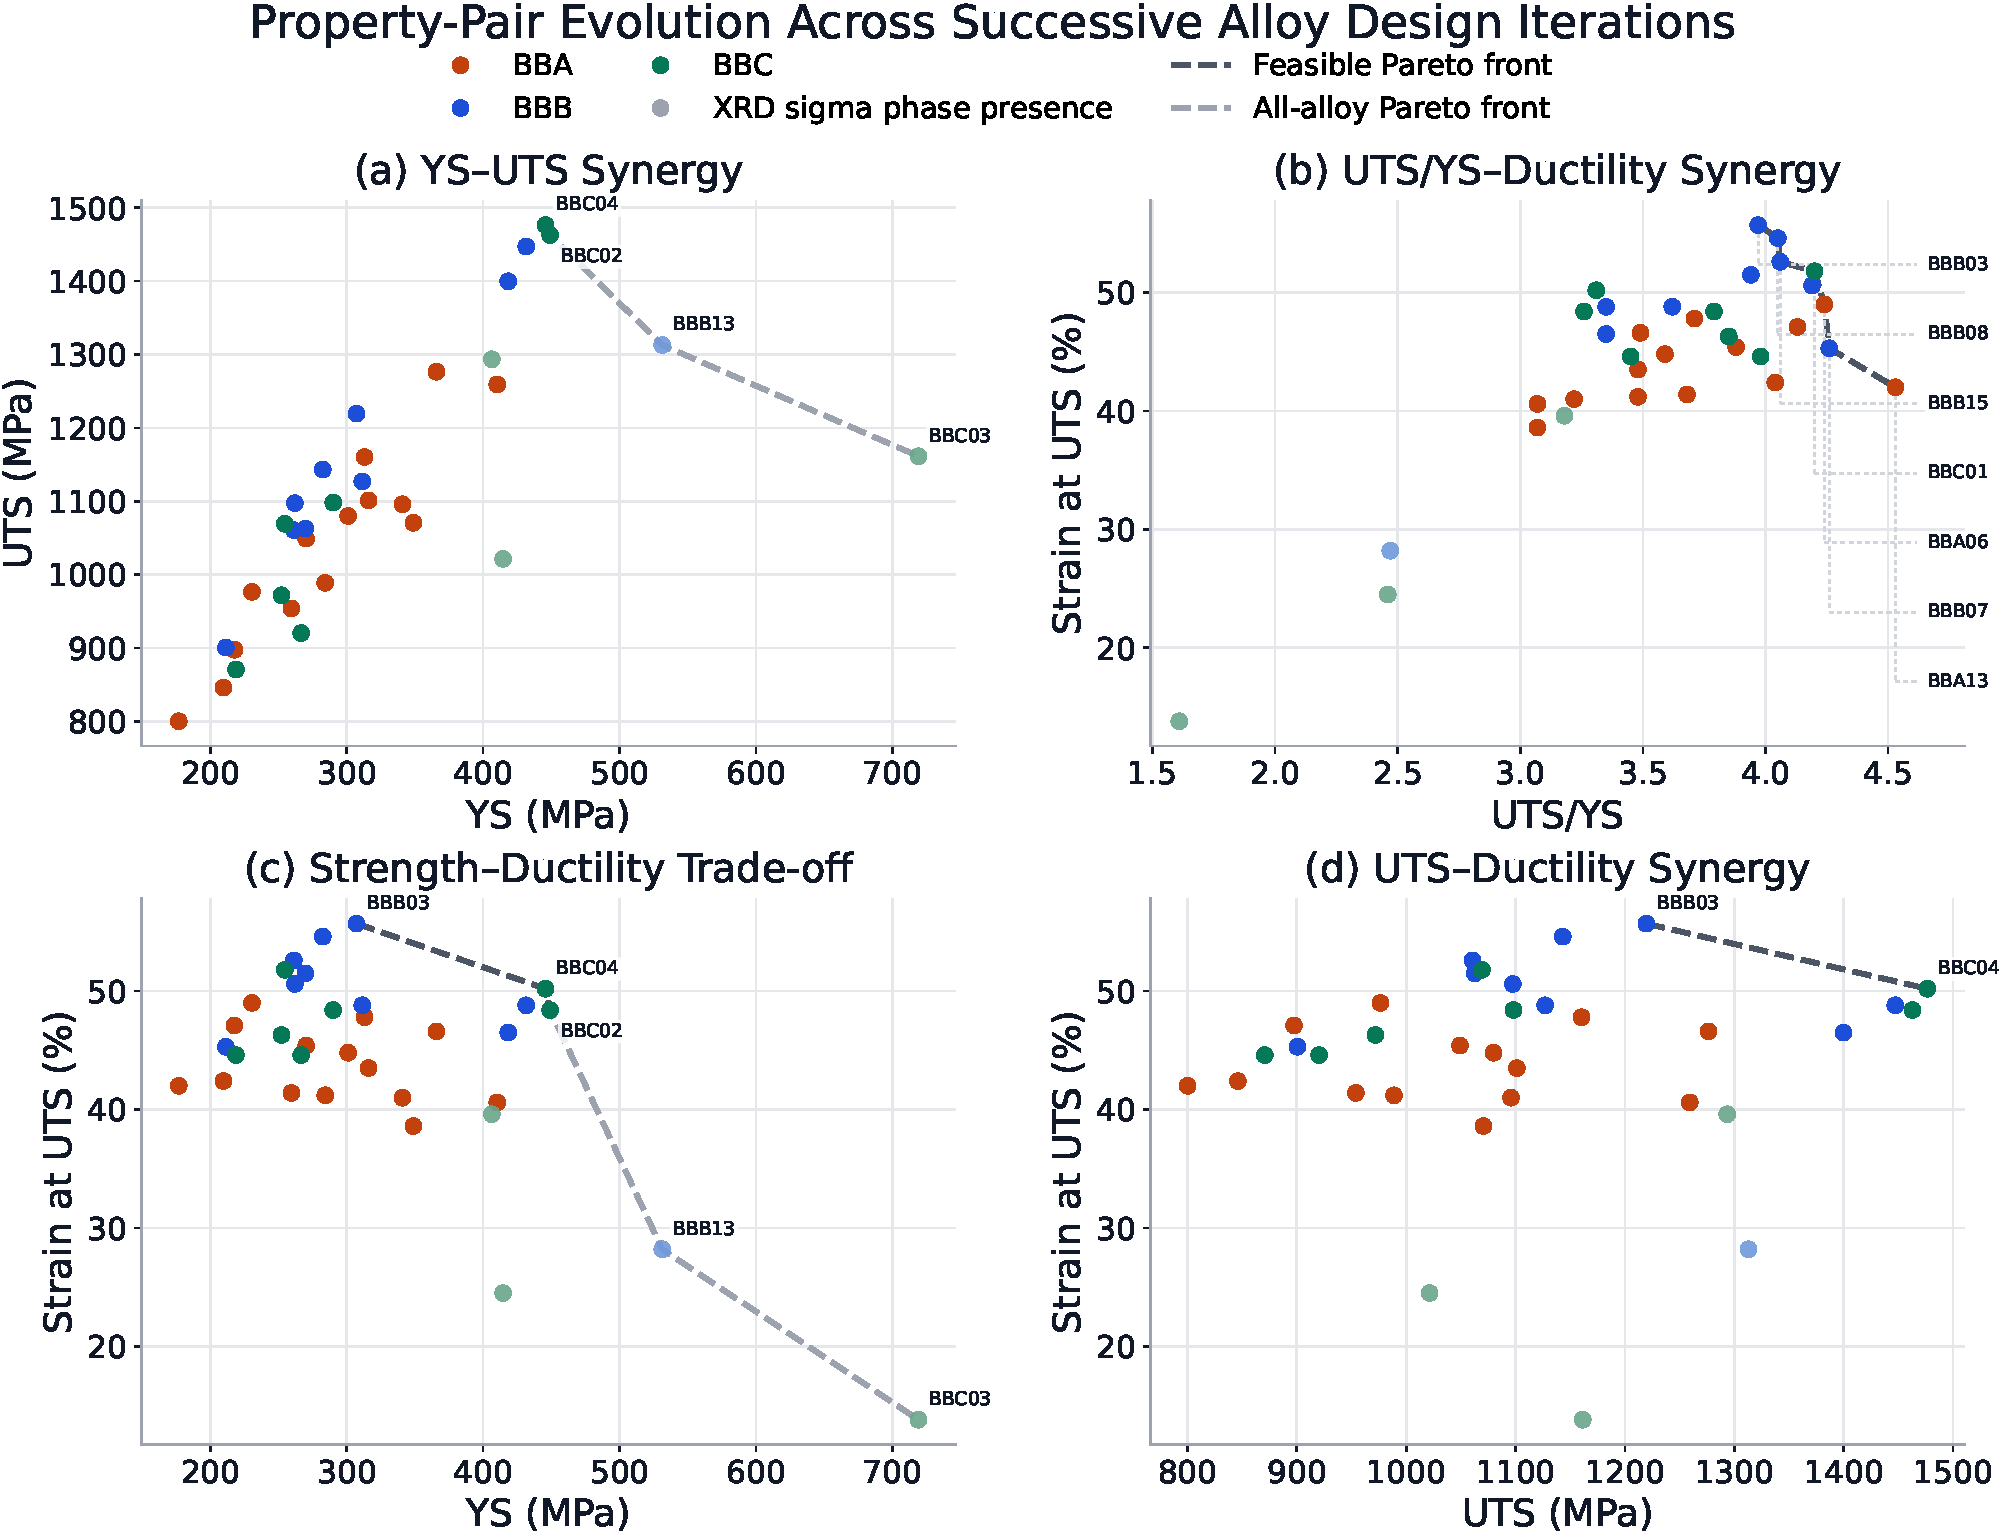
\includegraphics[width=\textwidth]{Figures/pair_plots.pdf}
    \caption{Pair plots of mechanical property combinations across three successive design iterations. Filled points denote single-phase FCC alloys and desaturated points indicate XRD-confirmed sigma phase presence. Dashed dark-grey lines trace the Pareto front considering only feasible alloys, while dashed light-grey lines trace the Pareto front considering all alloys.}
    \label{fig:pair_plots}
\end{figure*}

In panel~(a), most BBA (iteration~0) alloys occupy the lower-strength region, while BBB (iteration~1) and BBC (iteration~2) extend further into the upper-right portion of the plot. BBC04 reaches ${\sim}450$~MPa YS at ${\sim}1480$~MPa UTS, while BBC03 achieves ${\sim}720$~MPa YS but at lower UTS (${\sim}1160$~MPa), consistent with sigma-phase embrittlement. In panel~(b), several of the highest-ductility, highest-work-hardening alloys across the campaign, including BBB03, BBB08, BBB15, BBC01, and BBA06, cluster above 45\% elongation with UTS/YS $>$ 3.5. In panel~(c), the population follows the expected negative trend between elongation and YS, but BBC04 and BBC02 (${\sim}450$--490~MPa YS and ${\sim}48$--50\% elongation) sit above it. In panel~(d), BBB (iteration~1) and BBC (iteration~2) increasingly populate the upper-right quadrant, with BBC04 combining ${\sim}1480$~MPa UTS with ${\sim}50\%$ elongation.

The sigma-bearing alloys BBC03 and BBB13 serve as counterexamples: elevated YS comes at steep ductility cost, reinforcing the importance of phase stability as a design constraint. A detailed analysis of the compositional and microstructural factors driving these improvements will be presented in a forthcoming publication.

\subsubsection{Strength--DoP Correlations and Rate Sensitivity}

DoP shows the expected inverse correlation with strength metrics (\autoref{fig:DOPvAllStrengths}): higher YS and UTS correspond to lower penetration depth. The strong DoP--YS correlation ($r = -0.94$) raises the question of what DoP adds beyond YS alone. The residual variance captures the contribution of rate-dependent strengthening through the Cowper--Symonds constitutive model: alloys with the same YS but different rate-sensitivity exponents $m$ produce different DoP values, providing a simulation-derived discriminant that quasi-static testing alone cannot.

\begin{figure*}[t]
    \centering
    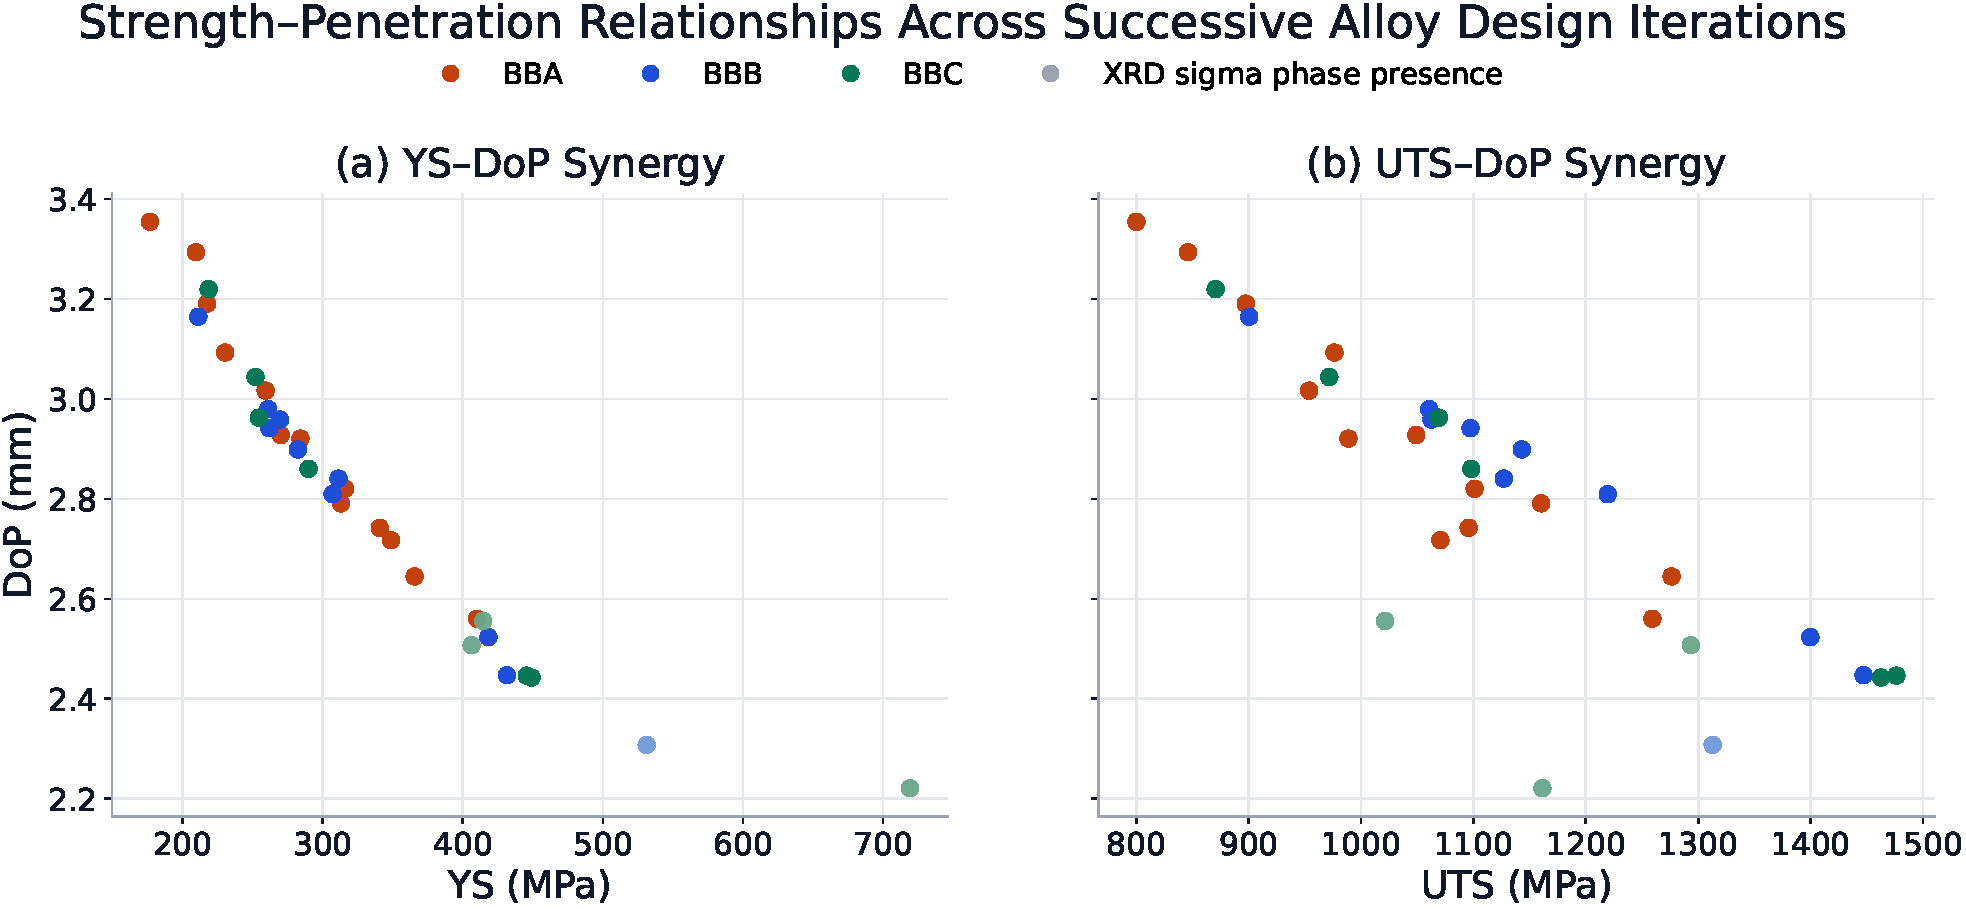
\includegraphics[width=0.8\textwidth]{Figures/Dop_vs_Strengths.pdf}
    \caption{Simulated depth of penetration (DoP) versus quasi-static strength metrics across all tested alloys: (a) yield strength (YS) and (b) ultimate tensile strength (UTS). In both panels, higher strength is associated with lower DoP, indicating that the strongest alloys also show the greatest simulated impact resistance.}
    \label{fig:DOPvAllStrengths}
\end{figure*}

The relationship between DoP and the calibrated rate-sensitivity exponent $m$ (\autoref{fig:MRelationships}(a)) is moderately positive, meaning that higher $m$ values are associated with larger penetration depths. YS and UTS both correlate negatively with $m$ (\autoref{fig:MRelationships}(b,c)), with the YS relationship stronger than the UTS relationship. Together, these trends indicate that alloys with higher quasi-static strength tend to exhibit lower calibrated rate-sensitivity exponents in this dataset, consistent with a trade-off between quasi-static strength and rate sensitivity in the present Cowper--Symonds fits.

\begin{figure*}[t]
    \centering
    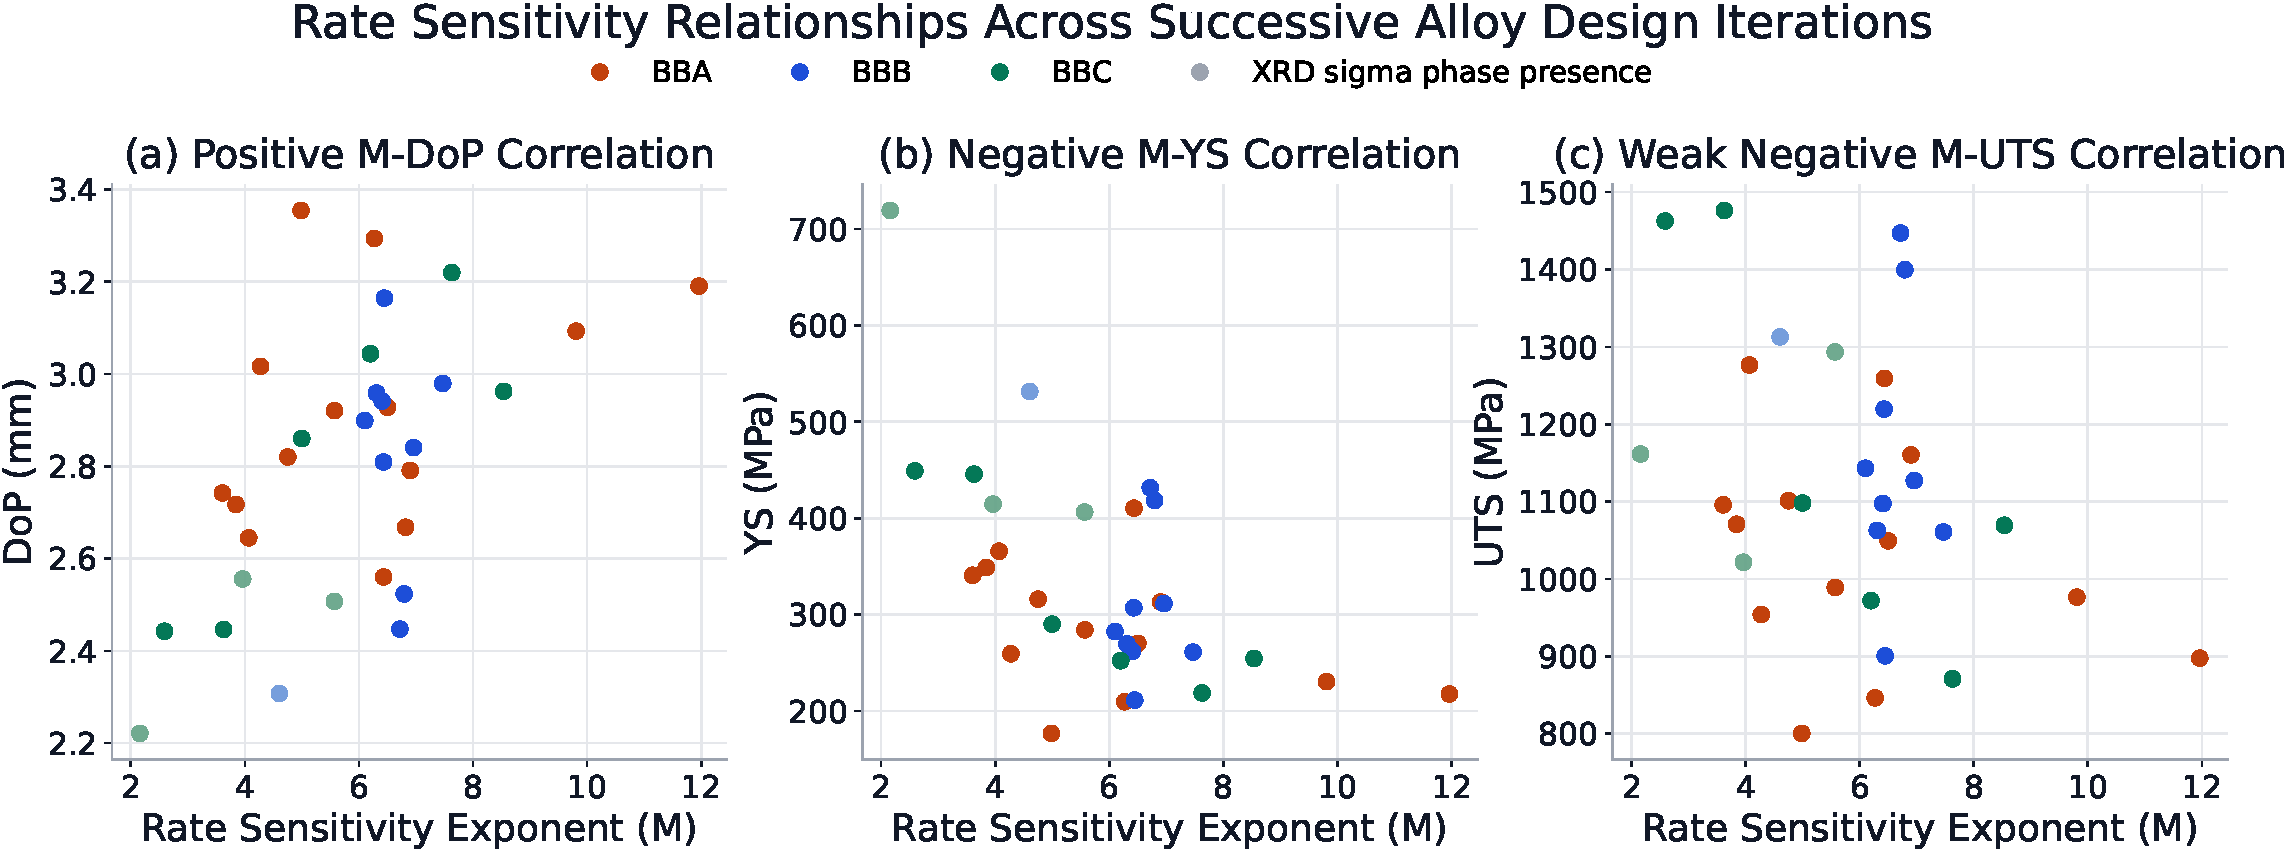
\includegraphics[width=0.9\textwidth]{Figures/M_plots.pdf}
    \caption{Rate sensitivity exponent ($m$) versus (a) simulated DoP, (b) yield strength, and (c) UTS for all candidate alloys across three iterations.}
    \label{fig:MRelationships}
\end{figure*}


\subsubsection{Emergent Compositional Design Rules}

The optimization campaign revealed two distinct compositional routes to high performance within the FCC-feasible space, which we describe below.

The first is a \emph{high-strength regime} defined by V = 20--24~at.\%, Cr $\leq$ 4~at.\%, Ni = 36--60~at.\%, and Cu = 0. The four strongest single-phase FCC alloys---BBC04 (${\sim}1480$~MPa UTS, 50\% elongation), BBC02 (${\sim}1460$~MPa, 48\%), BBB01 (${\sim}1450$~MPa, 49\%), and BBB12 (${\sim}1400$~MPa, 47\%)---all share this compositional signature. The strong V--YS correlation ($r = 0.82$, $n = 37$; Section~3.3.1) is consistent with lattice distortion strengthening from the large atomic-size and modulus mismatch of V in the FCC matrix~\cite{varvenne2016theory}. We note, however, that the Varvenne--Luque--Curtin model assumes a fully random solid solution; at V = 20--24~at.\%, deviations from randomness (short-range ordering or local V clustering) could affect quantitative agreement, and this has not been independently validated for the alloys in this campaign. Nickel stabilizes the FCC phase at high V concentrations (VEC effect), and chromium is minimized to avoid sigma formation. BBC04 is the most extreme example: 60~at.\% Ni and 24~at.\% V with no Co, no Cu, and only 4~at.\% Cr---an alloy at the outer edge of the design space that the BO identified precisely because the constraint-aware acquisition permitted boundary exploration.

The second is a \emph{high-ductility regime} with moderate V (8--12~at.\%), higher Mn (16~at.\%), and moderate Cr. BBB03 (${\sim}1220$~MPa UTS, 56\% elongation, UTS/YS = 3.97) and BBC01 (${\sim}1070$~MPa, 52\%, UTS/YS = 4.20) represent this compositional region. The elevated UTS/YS ratios and sustained elongation in these Mn-rich alloys are consistent with enhanced strain hardening, possibly through SFE reduction and twinning~\cite{li2016metastable, otto2013influences}, although direct microstructural evidence of the operating deformation mechanisms was not obtained in this campaign. These alloys trade peak strength for superior ductility and strain hardening capacity.

The two routes occupy different regions of the Pareto front and validate the 8-element expansion from Campaign~1. The high-strength route exploits V--Ni synergy that was inaccessible in the 6-element system (which lacked the compositional freedom to simultaneously maximize V and Ni while suppressing Cr). The high-ductility route exploits Mn, which was absent from Campaign~1 entirely. Cu, by contrast, showed negative Pearson correlations with all strength metrics ($r = -0.44$ to $-0.51$; Section~3.3.1) while its multi-objective corrSHAP is slightly positive ($r \approx +0.15$), reflecting partial cancellation across the five targets; it appeared in none of the top-performing alloys. The BO effectively learned to deprioritize Cu-containing compositions---a result that informs future campaign design in this alloy family.

\subsection{Bayesian Optimization Performance and Feasibility Analysis}

Sections 3.1--3.3 reported the properties and composition--property relationships across the three iterations. The optimization metrics below quantify how the BRAVE framework produced these outcomes, and what the pattern of successes and failures exposes about the structure of the constrained design problem.

Table~\ref{tab:bo_metrics} summarizes the optimization performance across the three iterations. The initial Pareto front (BBA) contained 10 non-dominated alloys with a hypervolume of 658.24. Iteration BBB increased the hypervolume to 817.77 (24.2\% gain) and expanded the Pareto front to 17 alloys, with 9 new non-dominated compositions. Iteration BBC reached a hypervolume of 856.30 (4.7\% gain) with 21 Pareto-optimal alloys.

The Bayesian advantage of the campaign is best measured by the concentration of experimental budget in high-value regions of the design space, rather than by Pareto front size or hypervolume trajectory---both of which are expected to increase under random sampling in correlated objective spaces. The campaign explored 0.12\% of the feasible space (33 feasible alloys out of 27,240 candidates) and concentrated four of its strongest alloys (BBC04, BBC02, BBB01, BBB12---all with V $\geq$ 20~at.\% and Ni $\geq$ 36~at.\%) in a compositional region comprising approximately 100 of the 27,240 feasible candidates ($<$0.4\% of the feasible space). Under random sampling, the probability of placing four or more of 33 draws in this region is $P \approx 6.5 \times 10^{-6}$ (hypergeometric distribution). The feasibility-weighted acquisition strategy is further validated by a controlled computational benchmark (Appendix), in which risk-weighted EHVI matched oracle performance (perfect feasibility knowledge) while reducing wasted evaluations approximately fivefold relative to feasibility-blind BO, across two bi-objective optimization problems on the 6-component Al--V--Cr--Fe--Co--Ni system.

\begin{table*}[t]
\centering
\caption{Bayesian Optimization Performance Across Iterations}
\label{tab:bo_metrics}
\begin{tabular}{lccccc}
\toprule
\textbf{Iteration} & \textbf{Avg EHVI} & \textbf{Hypervolume} & \textbf{HV Gain} & \textbf{Pareto Size} & \textbf{Infeasible} \\
\midrule
BBA & N/A & 658.24 & --- & 10 & 1/16 \\
BBB & 836.41 & 817.77 & 24.2\% & 17 (9 new) & 5/16 \\
BBC & 1059.2 & 856.30 & 4.7\% & 21 (5 new) & 9/16 \\
\bottomrule
\end{tabular}
\end{table*}

\subsubsection{Feasibility--Performance Trade-off}

The number of alloys infeasible for Bayesian optimization (sigma phase or manufacturing failure preventing XRD verification) increased across iterations: 1/16 in BBA (BBA04, manufacturing failure), 5/16 in BBB (BBB05, BBB06, BBB09, BBB11, BBB13---all sigma), and 9/16 in BBC (BBC03, BBC08, BBC14 sigma; BBC05, BBC06, BBC07, BBC09, BBC10, BBC16 failed cold rolling before XRD). Of the 33 FCC-confirmed alloys, most proceeded to full characterization. A few FCC-confirmed alloys (BBA09, BBB10, BBB16) showed mechanical anomalies (brittle fracture or processing-induced defects) that limited the quality of their objective data but did not change their phase classification.

\emph{Sigma-phase failures} decreased from 0 in BBA to 5 in BBB to 3 in BBC. The reduction from 5 to 3 between BBB and BBC reflects two mid-campaign interventions: the transition from TCHEA6 to TCHEA7 with dual-temperature screening, and the retraining of the GPC feasibility classifier on the 5 sigma outcomes from BBB. The GPC and updated CALPHAD screening reduced the sigma failure rate despite the BO continuing to target V-rich, high-strength compositions near the FCC/sigma boundary.

\emph{Manufacturing and processing failures} (alloys that never reached XRD verification or that failed during cold rolling) went from 1 in BBA to 0 in BBB to 6 in BBC. The six BBC processing failures all failed cold rolling. The current framework has no mechanism to predict or prevent these failures, as the GPC is trained only on phase outcomes. Post-hoc analysis suggests that V-containing nano-precipitates may be responsible for embrittlement in certain compositions, but this finding postdates the present study and will be reported separately.

This observation highlights a deeper tension in this alloy system. Table~\ref{tab:v_failure} quantifies the relationship between V content and outcome across all 48 alloys: no alloy with V = 0 failed, while failure rates exceed 50\% for V $\geq$ 12~at.\%. The top row of the performance landscape (V $\geq$ 20~at.\%) contains both the three strongest alloys in the campaign (BBC04, BBC02, BBB01---all at V = 24~at.\%) and four of the eight sigma-phase failures. At V = 24~at.\%, half the alloys fail and half are the best performers---the definition of a boundary-adjacent optimum. High V content simultaneously increases the risk of sigma-phase formation and processing-induced embrittlement. The highest-performing alloys therefore reside adjacent to multiple feasibility boundaries

\begin{table*}[t]
\centering
\caption{Failure rate and average yield strength by vanadium content across all 48 alloys.}
\label{tab:v_failure}
\small
\begin{tabular}{ccccp{0.48\textwidth}}
\toprule
\textbf{V (at.\%)} & \textbf{Total} & \textbf{Failed} & \textbf{Failure Rate} & \textbf{Notable Alloys} \\
\midrule
0  & 8  & 0 & 0\%   & --- \\
4  & 10 & 1 & 10\%  & BBA04 (manufacturing) \\
8  & 6  & 1 & 17\%  & BBC05 (cold rolling) \\
12 & 9  & 2 & 22\%  & BBC06, BBC07 (cold rolling) \\
16 & 4  & 4 & 100\% & BBB09, BBB11 (sigma); BBC10, BBC16 (cold rolling) \\
20 & 5  & 4 & 80\%  & BBB06, BBB13, BBC08 (sigma); BBC09 (cold rolling) \\
24 & 6  & 3 & 50\%  & BBB05, BBC03, BBC14 (sigma); BBC04, BBC02, BBB01 (FCC, top 3 UTS) \\
\bottomrule
\end{tabular}
\end{table*}

To quantify whether the relationship between V content and infeasibility is statistically significant, we applied two complementary tests~\cite{virtanen2020scipy}. First, treating V content as a continuous variable, the Pearson correlation between V content and infeasibility (coded as 0 or 1) is $r = 0.54$ ($P = 9.0 \times 10^{-5}$, $n = 48$): higher V is associated with higher probability of failure, and the probability that this association arises by chance is less than 0.01\%. This association is driven by V specifically, not by the V + Cr combination that defines the sigma stability threshold: V and Cr are uncorrelated across the 48 alloys ($r = 0.06$), confirming that V is a dominant predictor of infeasibility. Second, dividing alloys into high-V ($\geq 16$~at.\%) and low-V ($< 16$~at.\%) groups, 11 of 15 high-V alloys were infeasible compared to 4 of 33 low-V alloys---an odds ratio of 19.9 (Fisher's exact test, $P = 5.3 \times 10^{-5}$), meaning a high-V alloy is approximately 20 times more likely to fail than a low-V alloy. This association is robust to the choice of threshold: the odds ratio remains significant ($P < 0.05$) for all cutoffs from V $\geq$ 12 to V $\geq$ 20~at.\%.

Among the 30 feasible alloys with yield strength data, V content correlates with YS at $r = 0.84$ ($P = 8.7 \times 10^{-9}$). The same element that most strongly predicts mechanical performance also most strongly predicts failure---both at significance levels below $P < 10^{-4}$. The BO's preferential sampling of high-V alloys in iterations BBB and BBC (15 of 32 alloys with V $\geq$ 16~at.\%, compared to 0 of 16 in the diversity-sampled BBA) is itself evidence that the surrogates correctly identified V as the performance driver. The selection bias toward high V is not a confound---it is the optimizer doing its job, concentrating budget where the predicted payoff is highest. The consequence is that both the best alloys and the most failures accumulate in the same compositional region, which is the signature of a boundary-adjacent optimum.

This dual role is a pattern consistent with the general observation in constrained optimization that optimal solutions tend to lie on or near active constraint boundaries~\cite{ray2009infeasibility}. This coupling arises when the same compositional variable drives both performance and constraint violation: increasing V improves strength through lattice distortion effects (the objective gradient points toward high V) but simultaneously promotes sigma-phase formation (the constraint gradient points in the same direction). The unconstrained optimum would be a very high-V alloy that forms sigma. The constrained optimum is therefore the alloy with the highest V content that remains single-phase FCC---on the phase stability boundary by definition.

(Formally, the Karush--Kuhn--Tucker conditions for constrained optimality require $\nabla f + \lambda \nabla g = 0$ with multiplier $\lambda > 0$ at the solution, placing the optimum on the active constraint boundary $g(\mathbf{x}) = 0$~\cite{nocedal2006numerical}. The KKT conditions apply strictly to continuous, single-objective problems; the present campaign operates on a discrete compositional grid with multiple objectives, but the underlying intuition---that aligned objective and constraint gradients push optima toward boundaries---transfers to this setting.) If the optimum were far from the constraint, the constraint would not be restricting the search, and the problem would be effectively unconstrained. This has a practical implication for campaign design: in alloy systems where the primary strengthening element also destabilizes the target phase (e.g., V in the present system), a feasibility-aware acquisition strategy is a prerequisite for accessing the high-performing region of the design space. The present campaign provides an experimental realization of this principle: vanadium drives both the objective ($r = 0.84$ with YS) and the constraint ($r = 0.54$ with infeasibility), and the three strongest alloys in the campaign share the V = 24~at.\% boundary with three sigma failures. The boundary phenomenon has been observed implicitly in metastability-engineered HEAs, where optimal TRIP-mediated strength--ductility combinations arise at the edge of FCC phase stability~\cite{li2016metastable}, and has been proposed as an algorithmic strategy for constrained Bayesian optimization~\cite{tian2024boundary, maguire2025good}. However, the explicit connection between performance--constraint coupling through a shared compositional variable and the KKT prediction that constrained optima lie on active boundaries has not, to our knowledge, been demonstrated quantitatively in an experimental alloy campaign.

The sigma-phase trend (0 $\rightarrow$ 5 $\rightarrow$ 3) is the more informative metric for evaluating the feasibility-aware acquisition strategy. In iteration BBA, candidates were selected by diversity-aware k-medoids sampling across the interior of the FCC stability region, producing no sigma failures. In BBB, the BO targeted high-V, high-Cr regions where the GP surrogates predicted strong mechanical performance---the same regions where sigma is thermodynamically competitive. The 5 sigma failures provided the GPC with its first substantial training data and triggered the TCHEA7 transition. In BBC, the updated screening and retrained GPC reduced sigma failures to 3 despite continued exploration of the V-rich boundary---evidence that the feasibility-aware acquisition learned to avoid the most sigma-prone compositions while preserving access to the high-performing V-rich region.

The counterfactual remains instructive. A hard-filtered strategy would have excluded the high-V region entirely after the BBB sigma failures. BBC04 and BBC02---the two highest-UTS alloys in the campaign---would never have been synthesized. The BRAVE framework found them by accepting controlled risk near the phase boundary, with the GPC progressively sharpening the feasibility boundary between iterations.

The relevant performance metric is the performance gained per iteration, not the absolute failure rate. Despite 9/16 total failures in BBC (3 sigma + 6 processing), the 7 feasible alloys from that iteration included the strongest compositions in the campaign (BBC04, BBC02), and the hypervolume continued to increase (4.7\% gain over BBB). Extending the feasibility model to incorporate processing constraints---predicting which compositions are likely to fail cold rolling, independent of phase stability---is a priority for future campaigns.

The feasibility analysis also exposes CALPHAD database fidelity as a practical bottleneck for closed-loop alloy campaigns. The TCHEA6 database, used for initial screening, failed to predict sigma formation in several V- and Cr-rich compositions that were experimentally confirmed as multiphase. The mid-campaign transition to TCHEA7---with its expanded sigma, BCC, HCP, and liquid phase assessments across $>$100 ternary subsystems---reduced but did not eliminate these prediction errors (Section~3.1). The GPC feasibility classifier absorbs residual prediction errors by learning the empirical feasibility boundary from experimental phase outcomes, but its effectiveness depends on the quality of the thermodynamic screening that defines the initial candidate pool. A poorly calibrated CALPHAD database shifts the entire feasible space, potentially excluding high-performing regions from the outset or flooding the candidate pool with infeasible compositions that consume experimental budget before the GPC has sufficient training data to compensate. This dependency has practical implications: future campaigns should (i)~validate CALPHAD predictions against a small exploratory batch before committing to full-scale optimization, (ii)~incorporate dual-temperature screening (as we adopted here after iteration BBB) from the first iteration, and (iii)~prioritize thermodynamic databases with assessed coverage of the relevant ternary and quaternary subsystems.
